% Intended LaTeX compiler: pdflatex
\documentclass[bigger]{beamer}
\usepackage[utf8]{inputenc}
\usepackage[T1]{fontenc}
\usepackage{graphicx}
\usepackage{longtable}
\usepackage{wrapfig}
\usepackage{rotating}
\usepackage[normalem]{ulem}
\usepackage{amsmath}
\usepackage{amssymb}
\usepackage{capt-of}
\usepackage{hyperref}
\mode<beamer>{\usetheme{boxes}}
\mode<beamer>{\usepackage{amsmath}}
\usetheme{default}
\author{Konstantinos Papadimos}
\date{}
\title{Machine Learning Techniques in the Searches for Resonant Signatures at the LHC}
\hypersetup{
 pdfauthor={Konstantinos Papadimos},
 pdftitle={Machine Learning Techniques in the Searches for Resonant Signatures at the LHC},
 pdfkeywords={},
 pdfsubject={},
 pdfcreator={Emacs 28.2 (Org mode 9.5.5)}, 
 pdflang={English}}
\begin{document}

\maketitle

\section{Introductory stuff, Detectros and Particle physics}
\label{sec:org9c9d2c1}
\begin{frame}[label={sec:orgcd3de1b}]{The CMS Experiment overview}
\begin{figure}[hb]
\centering
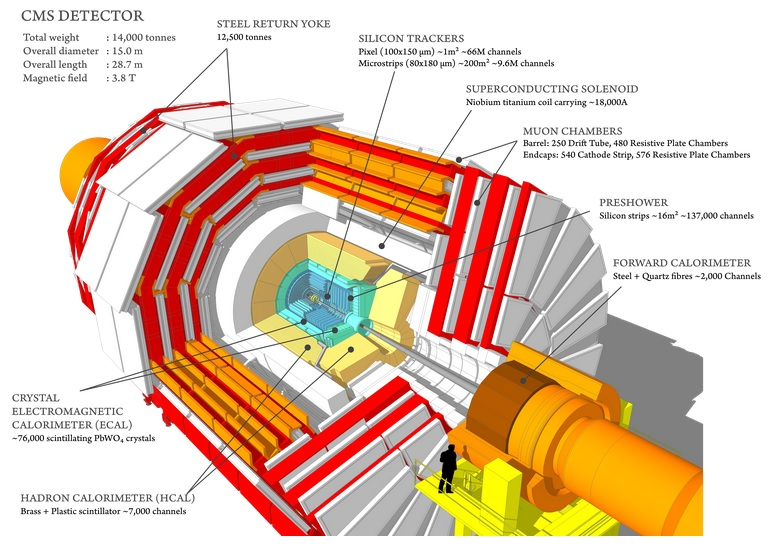
\includegraphics[width=\textwidth, ext=.png type=jpg]{/home/kpapad/UG_thesis/Thesis/Dissertation/src/figures/cms_detector.jpg}
\end{figure}
\end{frame}

\begin{frame}[label={sec:org5cabb5e}]{Coordinates at the CMS}
Given the solenoid geometry of the CMS detector, it is more convenient to use a spherical type of coordinates
\begin{equation}
\begin{matrix}
p_{x} = P_{T}\cos{\phi} \\
p_{y} = P_{T}\sin{\phi} \\
p_{z} = P_{T}\sinh{\eta}\\
|\vec{P}| = P_{T}\cosh{\eta} 
\end{matrix}
\end{equation}
\(\phi \in \left [ 0, 2\pi \right]\)the azimuthal angle, and \(\eta\in \left [ -\infty, +\infty \right ]\) is defined as:
\begin{equation}
\eta \equiv -\ln{\left [ \tan\left (\frac{\theta}{2} \right ) \right]  }
\end{equation}
\end{frame}

\begin{frame}[label={sec:orgb4188a6}]{Resonances}
\begin{figure}[hb]
\centering
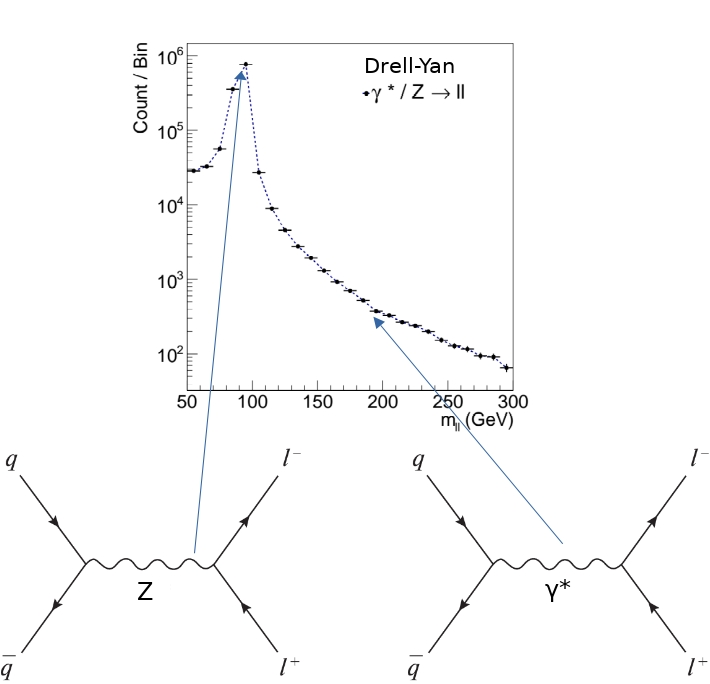
\includegraphics[width=0.75\textwidth, ext=.png type=jpg]{/home/kpapad/UG_thesis/Thesis/Dissertation/resonanceNONresonance.jpg}
\end{figure}
\end{frame}
\begin{frame}[label={sec:org59206de}]{Calibration and energy scale uncertainties}
\begin{block}{Why are resonances important?}
\begin{itemize}
\item They provide a way to probe and study the nature of particles produced at the LHC
\item We can calibrate the energy scale and resolution of the detector
\end{itemize}
\end{block}
\begin{block}{How do we calibrate the detector?}
\begin{itemize}
\item Calibration process adjusts energy scale and resolution to match well-known resonances (Z boson, J/psi meson) in data and simulation
\item Imperfect agreement due to subdetector complexities and nonlinear effects
\end{itemize}
\end{block}
\end{frame}
\begin{frame}[label={sec:orgec47dcd}]{Calibration and energy scale uncertainties}
\begin{block}{How do analysis techniques respond to energy scale uncertainties?}
Our work will focus on the effects that energy scale uncertainties have on a traditional fit-based analysis and a more modern Boosted Decision Tree-based analysis, using the generic diobject production process as the working example.
\end{block}
\end{frame}
\begin{frame}[label={sec:orgc9a7245}]{Calibration and energy scale uncertainties}
\begin{block}{In our case:}
\begin{itemize}
\item Signal: a resonant decay \(Y \rightarrow XX\)
\item Background: a non-resonant process
\end{itemize}
\end{block}
\begin{block}{How to separate them?}
\begin{itemize}
\item Boosted Decision Trees
\item Fit-based analysis
\end{itemize}
\end{block}
\end{frame}

\section{Analyis1: General Stuff}
\label{sec:orgd3bc825}
\begin{frame}[label={sec:org0f337df}]{Searches for \(Y \rightarrow XX\)}
\begin{columns}
\begin{column}{0.5\columnwidth}
Search for heavy \(Y \rightarrow XX\)
\begin{itemize}
\item Mass range from 100GeV up to 300GeV
\end{itemize}
\end{column}
\begin{column}{0.5\columnwidth}
Search for light \(Y \rightarrow XX\)
\begin{itemize}
\item Mass range from 50GeV up to 70GeV
\end{itemize}
\end{column}
\end{columns}
\end{frame}
\begin{frame}[label={sec:orgb6a3cdd}]{Methodology}
The specific characteristics(mass etc.) of each dataset  is different but the main idea is the same
\begin{itemize}
\item Background --> Drell-Yan
\item Signal --> \(W\Phi \rightarrow ll\)
\end{itemize}
\begin{figure}[hb]
\centering
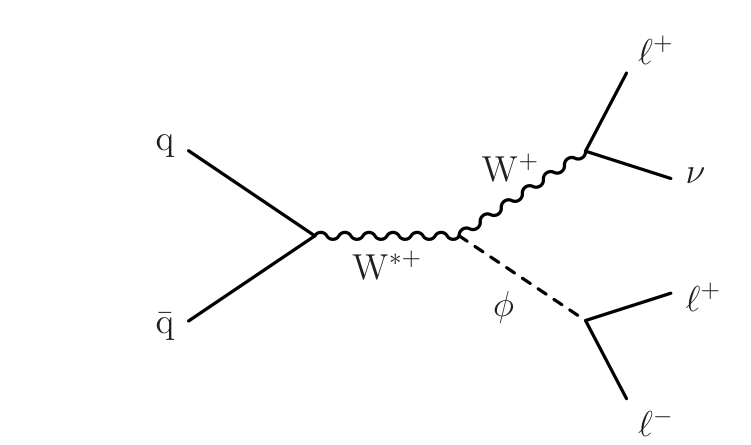
\includegraphics[width=0.7\textwidth, ext=.png]{/home/kpapad/UG_thesis/Thesis/Dissertation/2023-05-30-210442_751x445_scrot.png}
\end{figure}
\end{frame}

\begin{frame}[label={sec:org928b5c7}]{Methodology}
The specific characteristics(mass etc.) of each dataset  is different but the main idea is the same
\begin{itemize}
\item Background --> Drell-Yan
\item Signal --> \(W\Phi \rightarrow ll\)
\item Separate signal from background
\item Apply energy scale uncertainties to signal
\item Separate again
\item Compare the nominal case with the smeared cases
\end{itemize}
\end{frame}
\begin{frame}[label={sec:org069ca85}]{Statistical interpretation of results}
\alert{Are the signal events we counted, statistically significant?}
\begin{itemize}
\item We use the following metric:
\end{itemize}
\begin{equation}
\text{Significance} = \frac{Signal}{\sqrt{Background}}
\end{equation}
\end{frame}

\section{Light mass search}
\label{sec:orgcf1a404}
\begin{frame}[label={sec:org6dc42e6}]{Search for light \(Y \rightarrow XX\)}
We will study the following smearing cases:
\begin{columns}
\begin{column}{0.5\columnwidth}
\begin{itemize}
\item \(0\%\)(Nominal case)
\item \(5\%\)
\item \(7\%\)
\item \(10\%\)
\item \(12\%\)
\end{itemize}
The working mass range is quite small --> smearing has a significant effect real quick.
\end{column}
\begin{column}{0.5\columnwidth}
\begin{figure}[h]
\centering
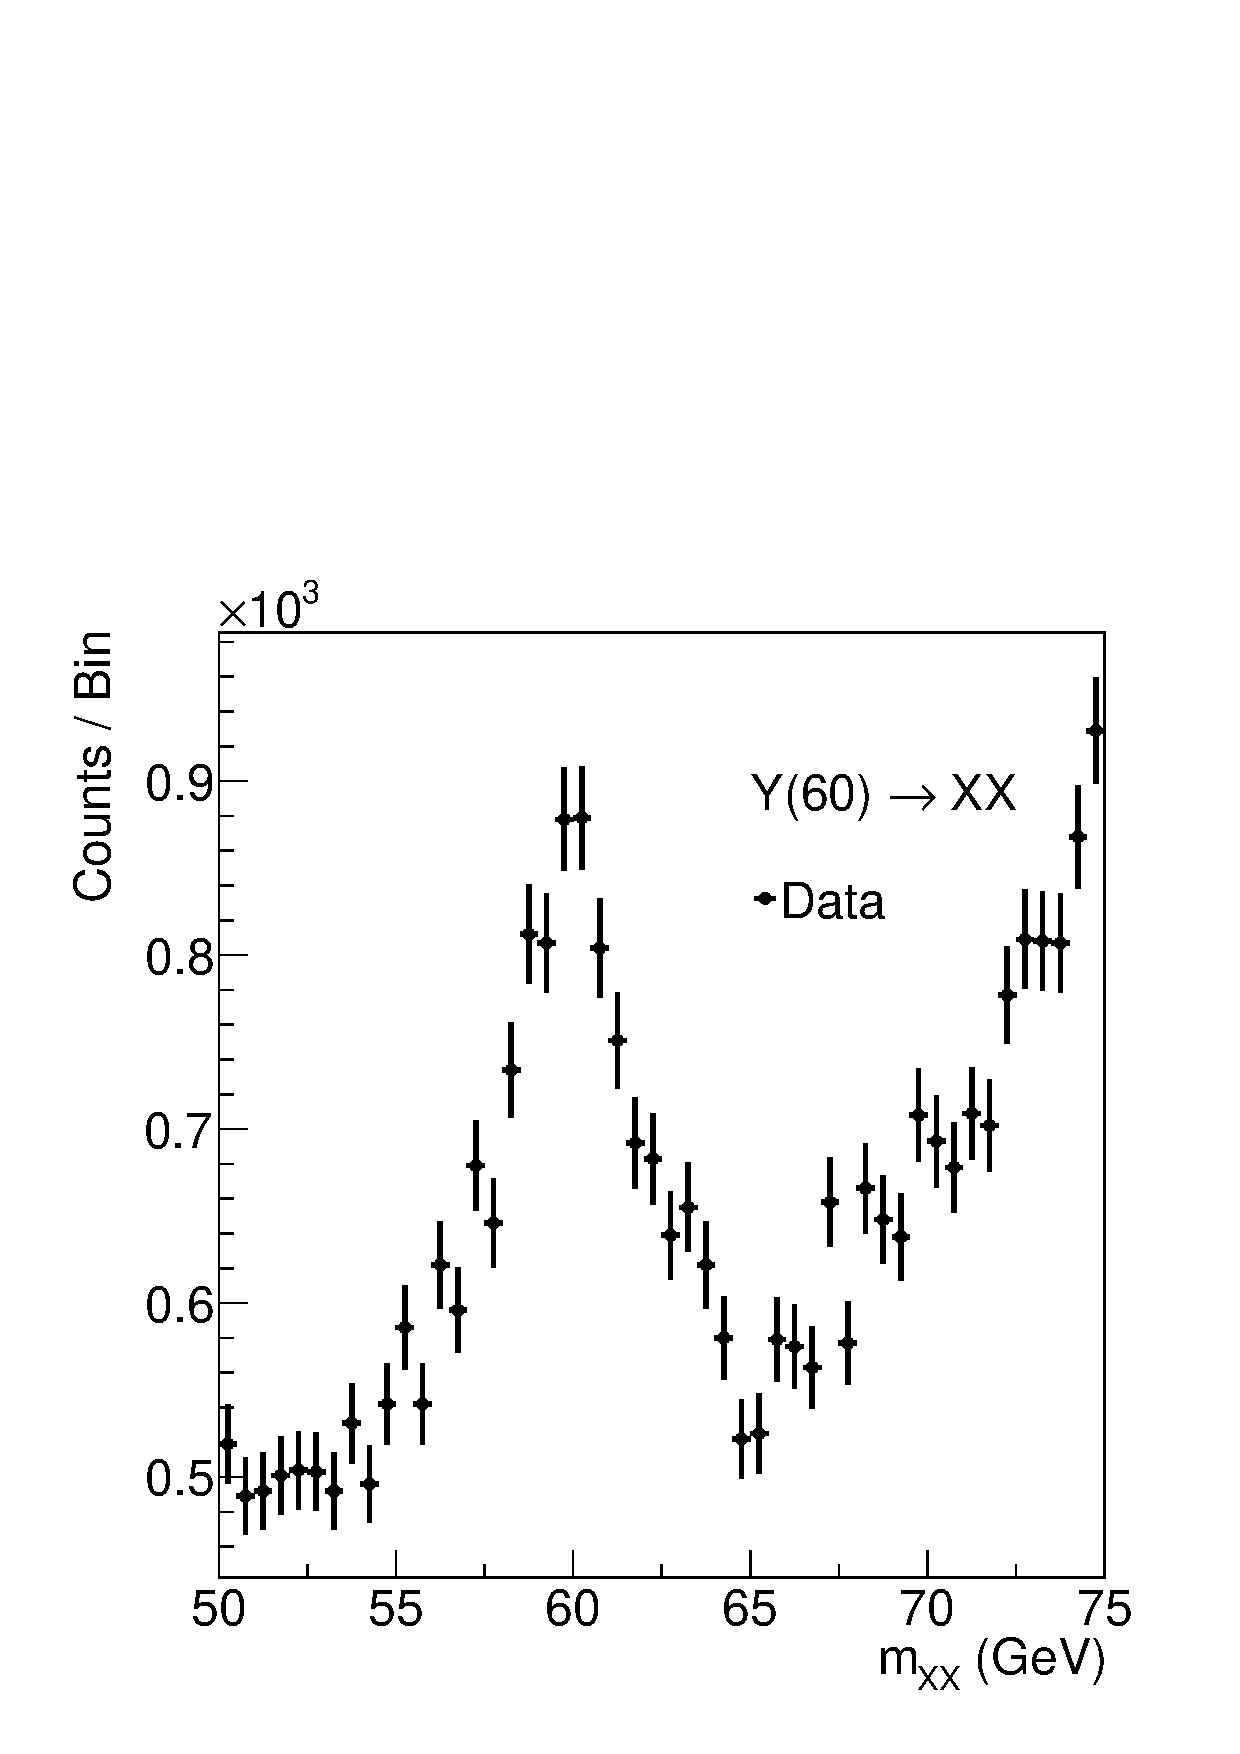
\includegraphics[page=1,width=\textwidth]{/home/kpapad/UG_thesis/Thesis/Analysis/out/Plots/WPhiJets_M60M5080_Application_MassSpectrum.pdf}
\end{figure}
\end{column}
\end{columns}
\end{frame}
\begin{frame}[label={sec:orgf8766d4}]{Fit based signal from background separation}
To fit the mass spectrum we use a background component\ldots{}
\begin{figure}[hb]
\centering
\includegraphics[page=2, width=0.5 \textwidth, ext=.png type=jpg]{/home/kpapad/UG_thesis/Thesis/Analysis/src/WPhiJets_M60M5080_SampleFitWArrows.pdf}
\end{figure}
\end{frame}
\begin{frame}[label={sec:org7bc0b4a}]{Fit based signal from background separation}
\ldots{} and a signal component \ldots{}
\begin{figure}[hb]
\centering
\includegraphics[page=3, width=0.5 \textwidth, ext=.png type=jpg]{/home/kpapad/UG_thesis/Thesis/Analysis/src/WPhiJets_M60M5080_SampleFitWArrows.pdf}
\end{figure}
\end{frame}
\begin{frame}[label={sec:org79afe46}]{Fit based signal from background separation}
\ldots{} Signal + Background = Mass spectrum
\begin{figure}[hb]
\centering
\includegraphics[page=4, width=0.5 \textwidth, ext=.png type=jpg]{/home/kpapad/UG_thesis/Thesis/Analysis/src/WPhiJets_M60M5080_SampleFitWArrows.pdf}
\end{figure}
\end{frame}

\begin{frame}[label={sec:org6820dc5}]{Fit based approach: Fitting}
Then we proceed with the fits!
\begin{columns}
\begin{column}{0.5\columnwidth}
\begin{figure}[h]
\centering
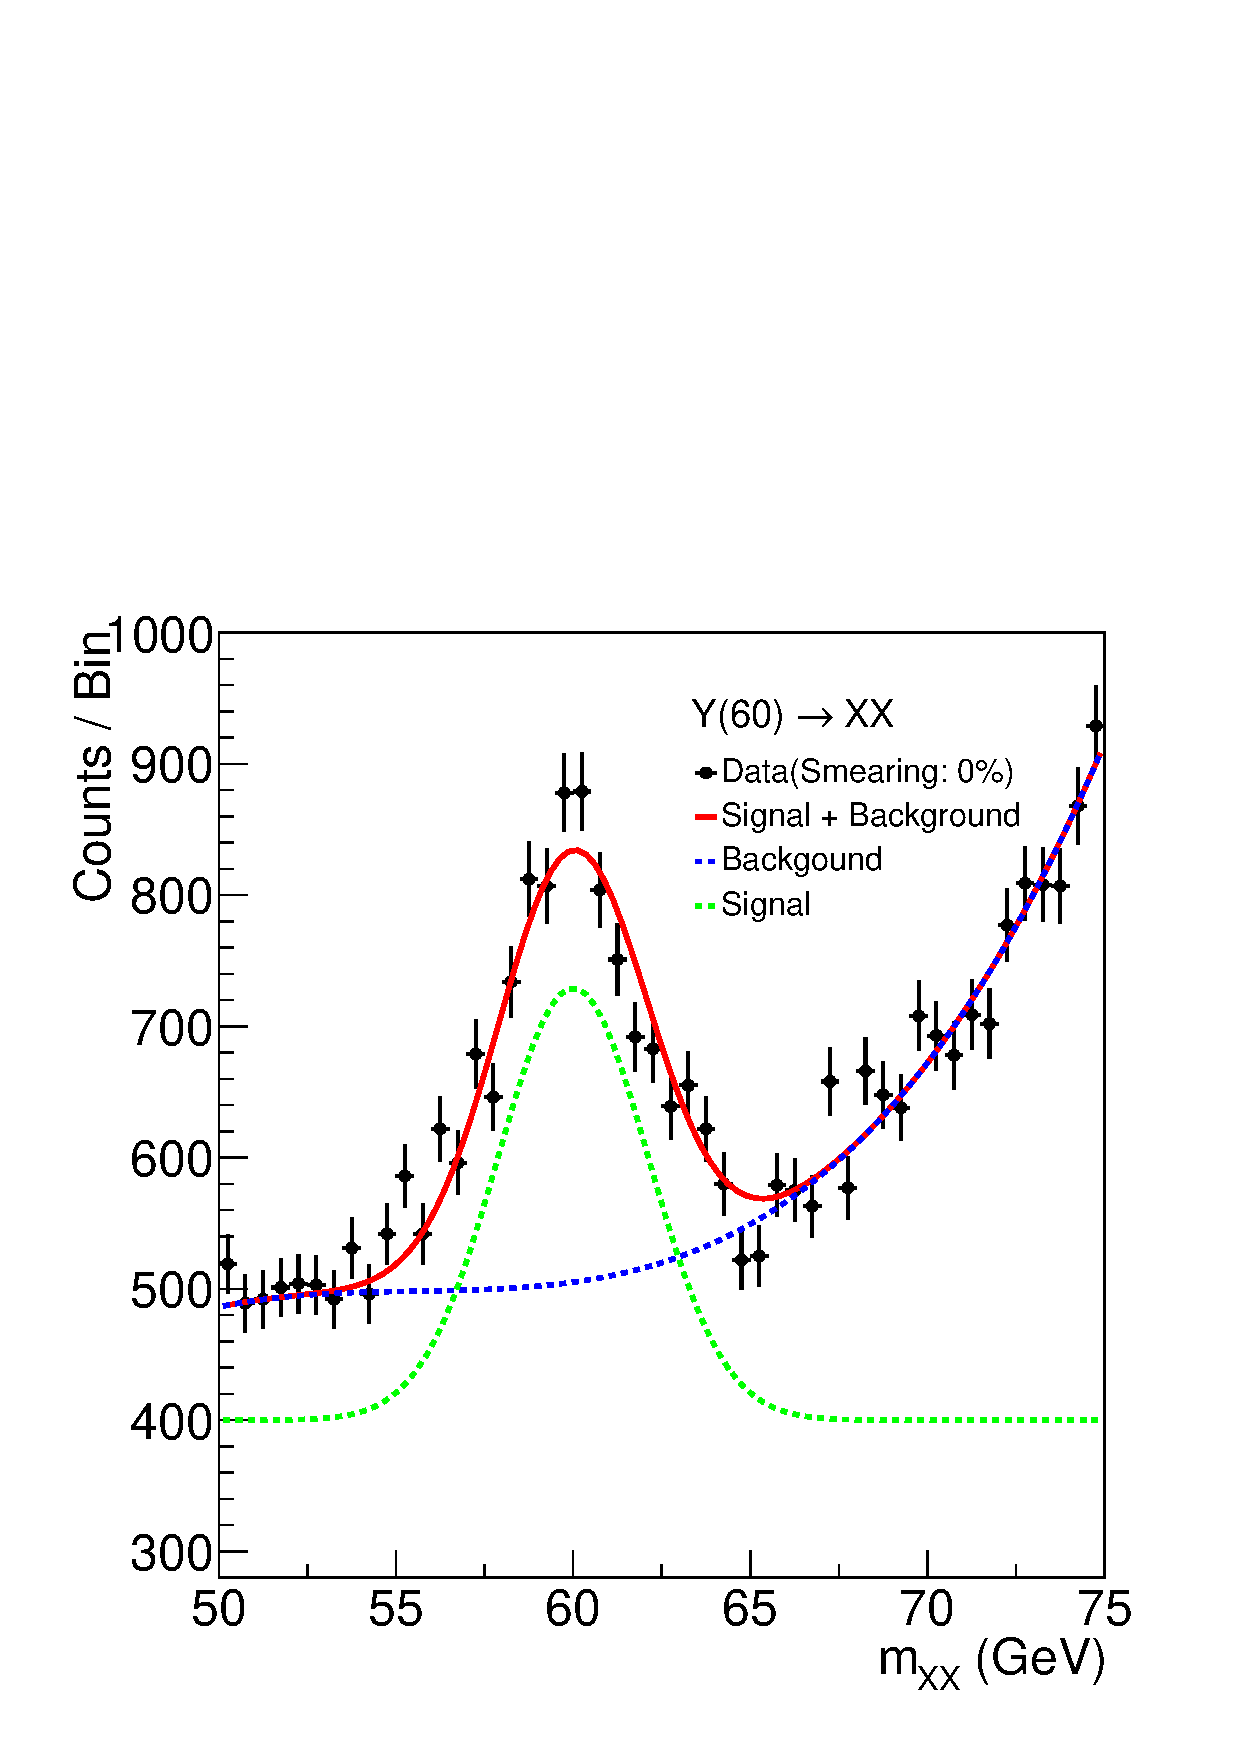
\includegraphics[page=1,width=\linewidth]{/home/kpapad/UG_thesis/Thesis/Analysis/src/WPhiJets_M60M5080_FitALL.pdf}
\end{figure}
\end{column}

\begin{column}{0.5\columnwidth}
\begin{figure}[h]
\centering
\includegraphics[page=2,width=\linewidth]{/home/kpapad/UG_thesis/Thesis/Analysis/src/WPhiJets_M60M5080_FitALL.pdf}
\end{figure}
\end{column}
\end{columns}
\end{frame}

\begin{frame}[label={sec:orgf75ed2c}]{Fit based approach: Fitting}
\begin{columns}
\begin{column}{0.5\columnwidth}
\begin{figure}[h]
\centering
\includegraphics[page=3,width=\linewidth]{/home/kpapad/UG_thesis/Thesis/Analysis/src/WPhiJets_M60M5080_FitALL.pdf}
\end{figure}
\end{column}

\begin{column}{0.5\columnwidth}
\begin{figure}[h]
\centering
\includegraphics[page=4,width=\linewidth]{/home/kpapad/UG_thesis/Thesis/Analysis/src/WPhiJets_M60M5080_FitALL.pdf}
\end{figure}
\end{column}
\end{columns}
\end{frame}

\begin{frame}[label={sec:org62ba991}]{Fit based approach: Fitting}
Any further smearing will make the signal indistinguishable!
\begin{figure}[h]
\centering
\includegraphics[page=5,width=0.55\textwidth]{/home/kpapad/UG_thesis/Thesis/Analysis/src/WPhiJets_M60M5080_FitALL.pdf}
\end{figure}
\end{frame}

\begin{frame}[label={sec:org280ef13}]{Fit based approach: Signal from background separation}
Working in the nominal case, we find the region that yields the best significance, by scanning the ranges. \(m=\pm \frac{n}{2}\sigma\text{, }n=1, 2, 3, 4, 5, 6\) 
\begin{figure}[h]
\centering
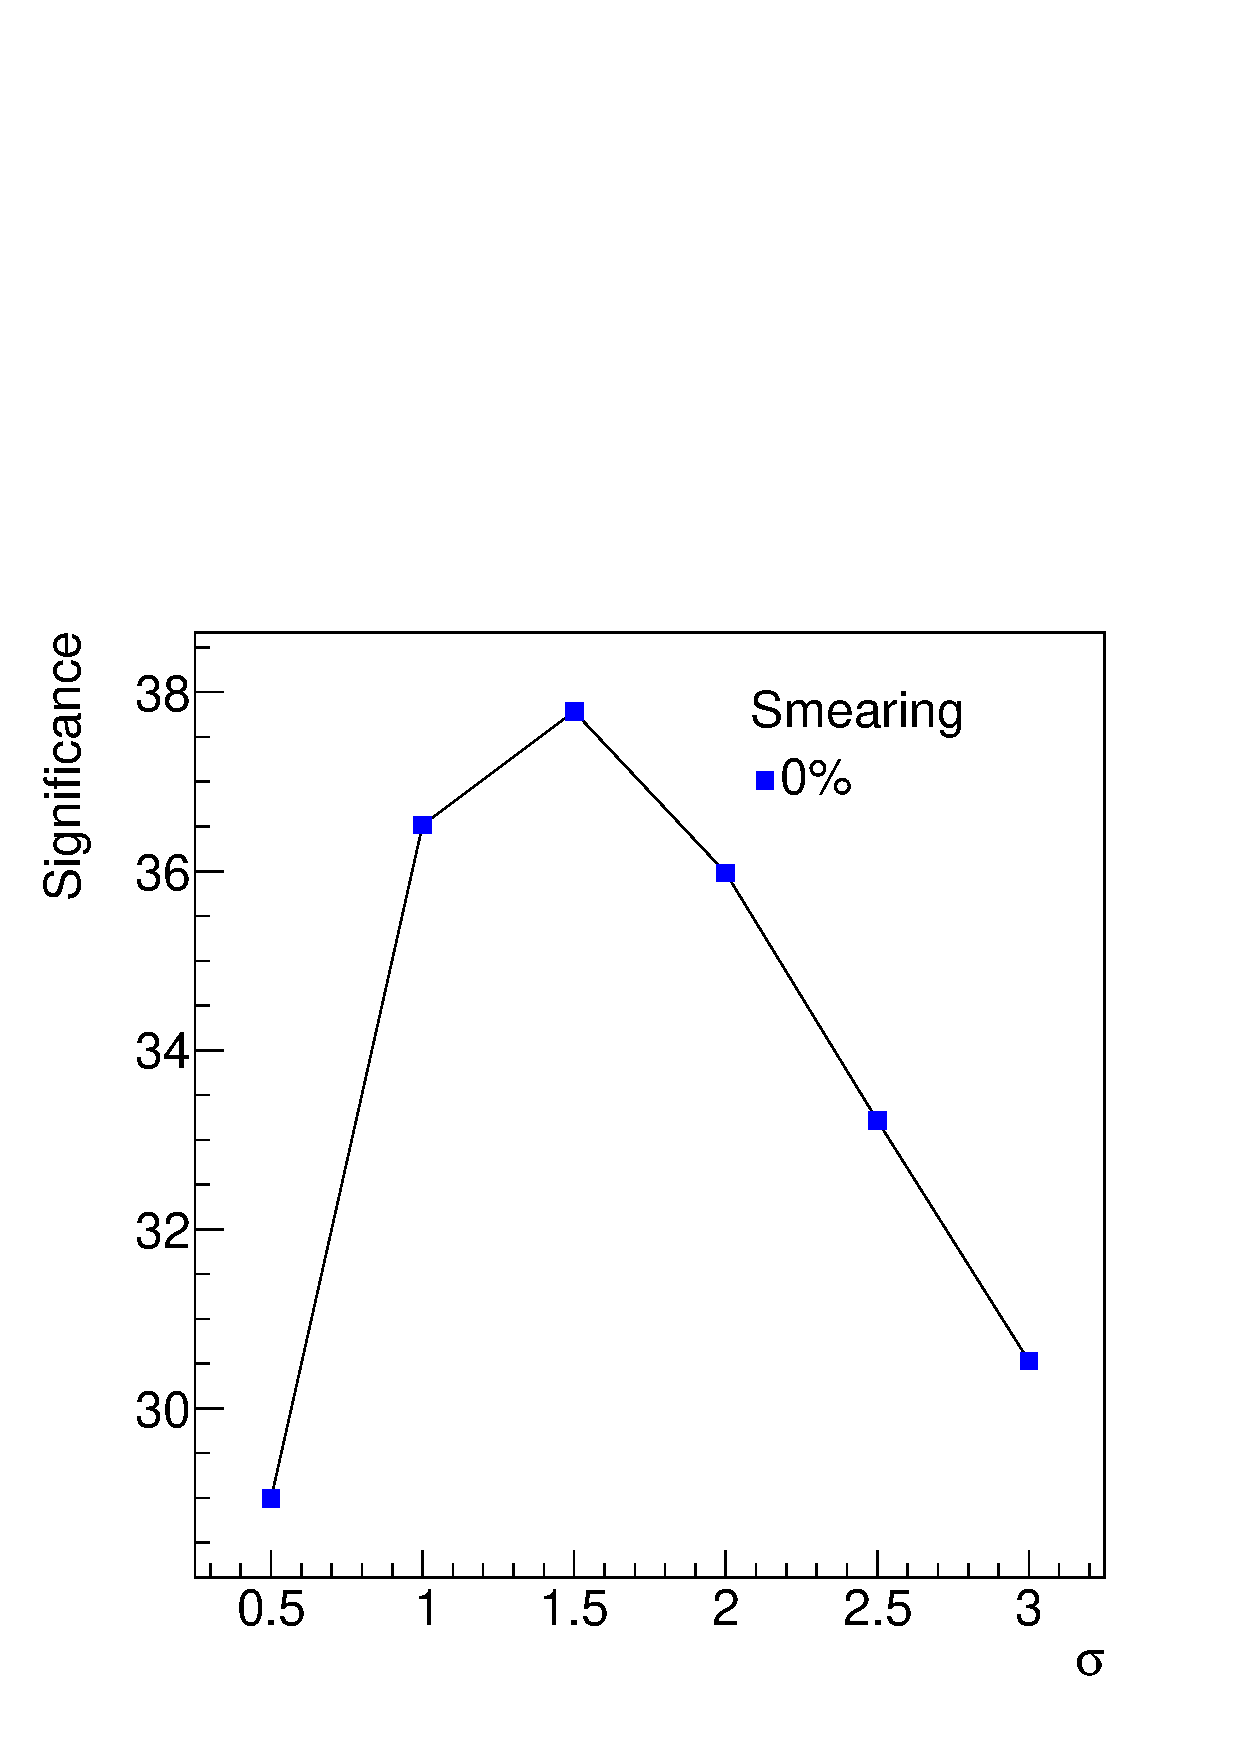
\includegraphics[page=1,width=0.45\linewidth]{/home/kpapad/UG_thesis/Thesis/Analysis/src/WPhiJets_M60M5080_Significance0.pdf}
\end{figure}
\end{frame}
\begin{frame}[label={sec:orgfbf0dda}]{Fit based approach: Signal from background separation}
\begin{columns}
\begin{column}{0.5\columnwidth}
\begin{figure}[h]
\centering
\includegraphics[page=3,width=\linewidth]{/home/kpapad/UG_thesis/Thesis/Analysis/src/WPhiJets_M60M5080_MassWinodwShow.pdf}
\end{figure}
\end{column}
\begin{column}{0.5\columnwidth}
\begin{figure}[h]
\centering
\includegraphics[page=3,width=\linewidth]{/home/kpapad/UG_thesis/Thesis/Analysis/src/WPhiJets_M60M5080_MassWinodwShow2.pdf}
\end{figure}
\end{column}
\end{columns}
\end{frame}
\begin{frame}[label={sec:org113fb2a}]{Fit based approach: Signal from background separation}
\begin{figure}[h]
\centering
\includegraphics[page=3,width=0.6\linewidth]{/home/kpapad/UG_thesis/Thesis/Bdt/src/WPhiJets_M60M5080_Significance.pdf}
\end{figure}
\end{frame}
\begin{frame}[label={sec:org85ebbd8}]{BDT approach: Feature space}
\alert{What features of the dataset are best for the classification task?}
\begin{figure}[h!]
\centering
\includegraphics[page=1,width=0.9\textwidth]{/home/kpapad/UG_thesis/Thesis/Analysis/out/Plots/WPhiJets_M60M5080DeltasVarsPlots.pdf}
\end{figure}
\end{frame}
\begin{frame}[label={sec:orgfbef1ad}]{BDT approach: Feature space}
\begin{figure}[h!]
\centering
\includegraphics[page=2,width=0.9\textwidth]{/home/kpapad/UG_thesis/Thesis/Analysis/out/Plots/WPhiJets_M60M5080DeltasVarsPlots.pdf}
\end{figure}
\end{frame}

\begin{frame}[label={sec:orgf637bac}]{BDT approach: The model}
\begin{columns}
\begin{column}{0.5\columnwidth}
\begin{itemize}
\item Trained with approximately 3K events.
\item To examine overfitting we compare the ratio of training events to testing for each bdt score
\end{itemize}
\end{column}
\begin{column}{0.5\columnwidth}
  \begin{figure}[h!]
\centering
\includegraphics[page=5, width=\textwidth]{/home/kpapad/UG_thesis/Thesis/Bdt/out/Plots/WPhiJets_M60M5080DeltasPConf13BDTplot.pdf}
\end{figure}
\end{column}
\end{columns}
\end{frame}

\begin{frame}[label={sec:orgb0d2a7d}]{BDT approach: Application}
Feed the application set to the BDT --> BDT plots
\begin{columns}
\begin{column}{0.5\columnwidth}
\begin{figure}[h]
\centering
\includegraphics[page=6,width=\linewidth]{/home/kpapad/UG_thesis/Thesis/Bdt/out/Plots/WPhiJets_M60M5080Deltas_Application13BDTplot.pdf}
\end{figure}
\end{column}
\begin{column}{0.5\columnwidth}
\begin{figure}[h]
\centering
\includegraphics[page=6,width=\linewidth]{/home/kpapad/UG_thesis/Thesis/Bdt/out/Plots/WPhiJets_M60M5080Deltas_Application_Smeared513BDTplot.pdf}
\end{figure}
\end{column}
\end{columns}
\end{frame}

\begin{frame}[label={sec:orgdf56697}]{BDT approach: Application}
\begin{columns}
\begin{column}{0.5\columnwidth}
\begin{figure}[h]
\centering
\includegraphics[page=6,width=\linewidth]{/home/kpapad/UG_thesis/Thesis/Bdt/out/Plots/WPhiJets_M60M5080Deltas_Application_Smeared713BDTplot.pdf}
\end{figure}
\end{column}
\begin{column}{0.5\columnwidth}
\begin{figure}[h]
\centering
\includegraphics[page=6,width=\linewidth]{/home/kpapad/UG_thesis/Thesis/Bdt/out/Plots/WPhiJets_M60M5080Deltas_Application_Smeared1013BDTplot.pdf}
\end{figure}
\end{column}
\end{columns}
\end{frame}

\begin{frame}[label={sec:org2ec8d2c}]{BDT approach: Application}
\begin{columns}
\begin{column}{0.5\columnwidth}
\begin{figure}[h]
\centering
\includegraphics[page=6,width=\linewidth]{/home/kpapad/UG_thesis/Thesis/Bdt/out/Plots/WPhiJets_M60M5080Deltas_Application_Smeared1213BDTplot.pdf}
\end{figure}
\end{column}
\end{columns}
\end{frame}

\begin{frame}[label={sec:orgd34a4be}]{BDT approach: Signal from background separation}
\alert{Where should we place the cut?}
\begin{columns}
\begin{column}{0.5\columnwidth}
\begin{itemize}
\item Same philosophy as in the fit based search
\item We scan the bdt range to find the best region of interest
\item Best cut --> BDT score = 0.96.
\end{itemize}
\end{column}
\begin{column}{0.5\columnwidth}
\begin{figure}
\centering
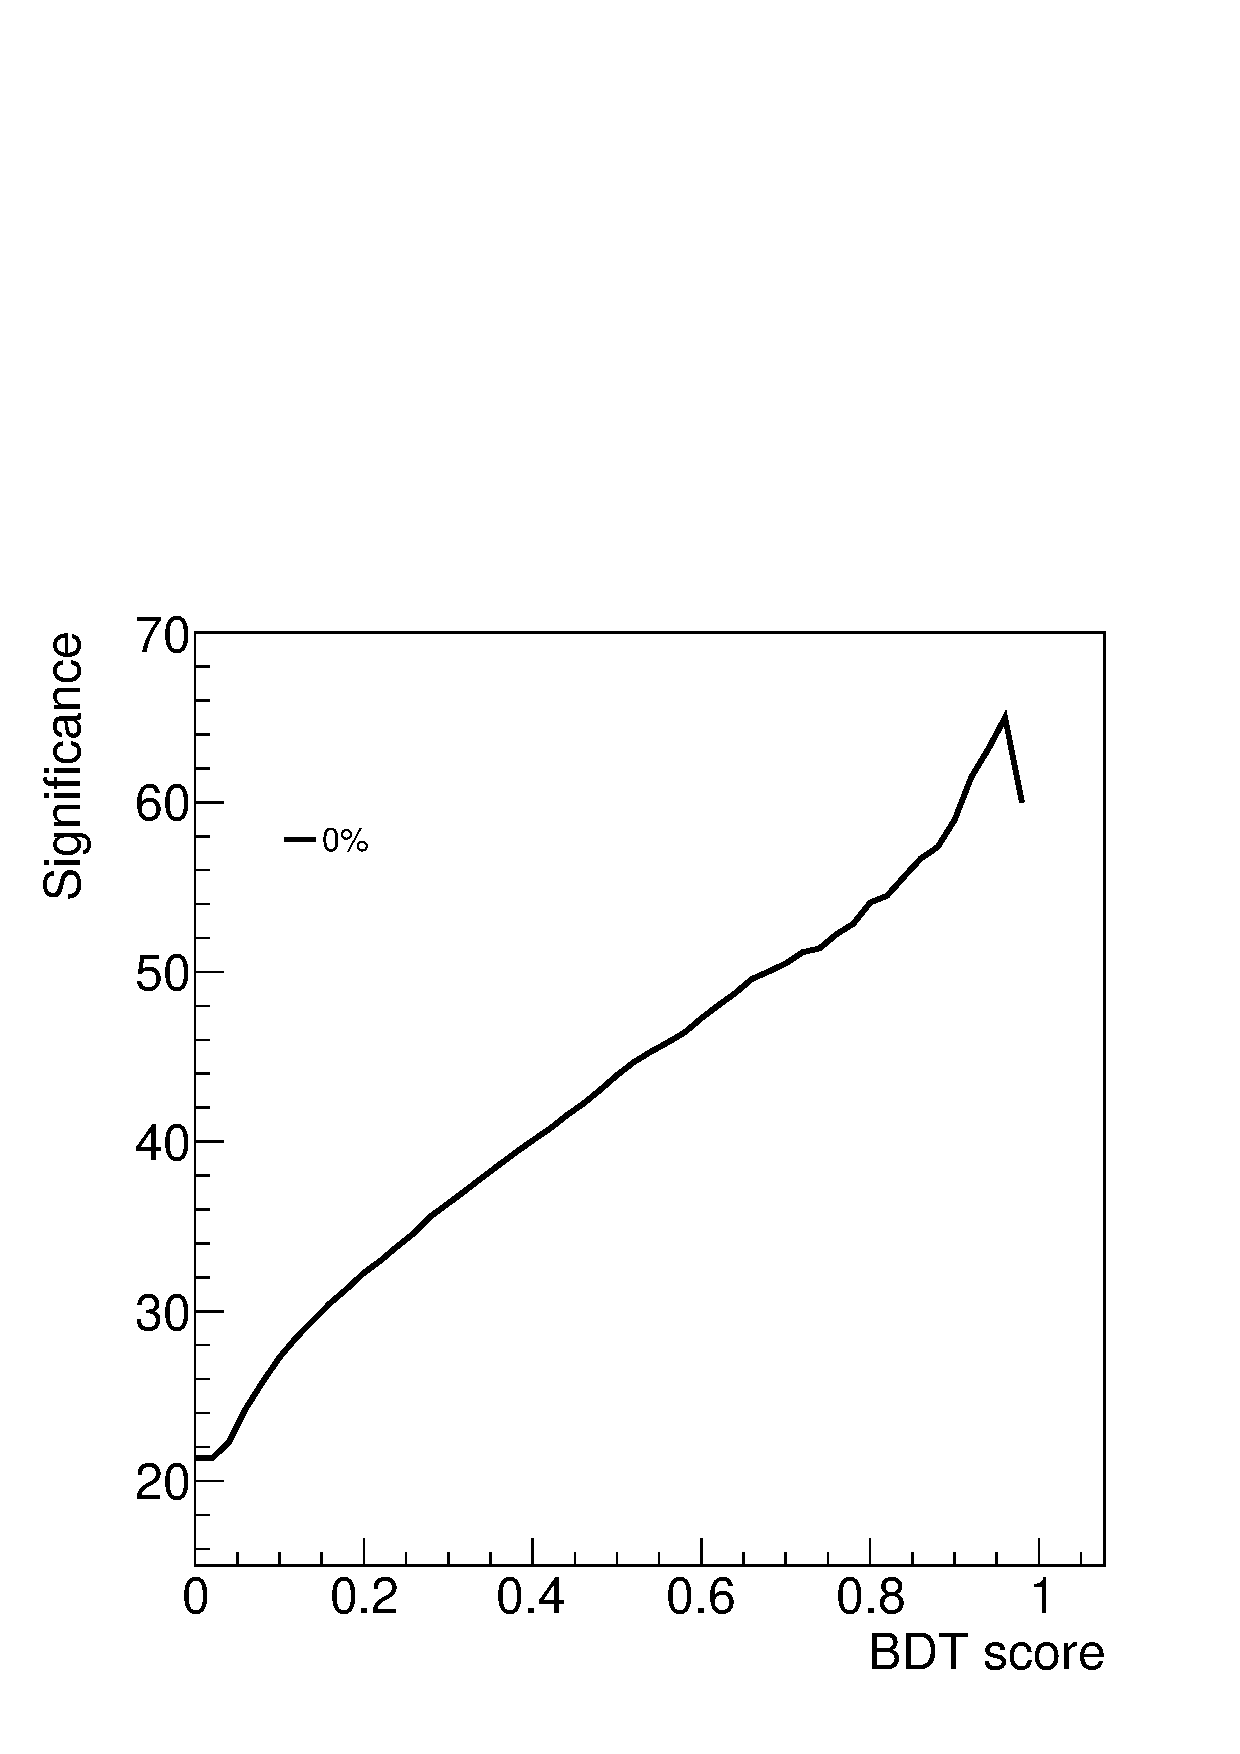
\includegraphics[page=1,width=\linewidth]{/home/kpapad/UG_thesis/Thesis/Bdt/src/WPhiJets_M60M5080_Significance0bdt.pdf}
\end{figure}
\end{column}
\end{columns}
\end{frame}
\begin{frame}[label={sec:orgaffe3b5}]{BDT approach: Signal from background separation}
\begin{columns}
\begin{column}{0.5\columnwidth}
\begin{itemize}
\item The performance of the BDT remains invariant under energy scale uncertainties!
\end{itemize}
\end{column}
\begin{column}{0.5\columnwidth}
\begin{figure}
\centering
\includegraphics[page=2,width=\textwidth]{/home/kpapad/UG_thesis/Thesis/Bdt/src/WPhiJets_M60M5080_Significance.pdf}
\end{figure}
\end{column}
\end{columns}
\end{frame}
\begin{frame}[label={sec:orgb9c7d05}]{Synopsis}
\begin{columns}
\begin{column}{0.5\columnwidth}
\begin{itemize}
\item BDT performs better than the fit-based.
\item Remains invariant under smearing.
\item Performance of the fit drops.
\end{itemize}
\end{column}
\begin{column}{0.5\columnwidth}
\begin{figure}
\centering
\includegraphics[page=4,width=\textwidth]{/home/kpapad/UG_thesis/Thesis/Bdt/src/WPhiJets_M60M5080_Significance.pdf}
\end{figure}
\end{column}
\end{columns}
\end{frame}

\section{Heavy mass search}
\label{sec:org03fa458}
\begin{frame}[label={sec:org0fecfb2}]{Search for heavy \(Y \rightarrow XX\)}
We will study the following smearing cases:\newline

\begin{columns}
\begin{column}{0.5\columnwidth}
Medium to extreme cases
\begin{itemize}
\item \(0\%\)(Nominal case)
\item \(5\%\)
\item \(10\%\)
\item \(15\%\)
\item \(20\%\)
\end{itemize}
\newline Plus some really extreme cases
\begin{itemize}
\item \(30\%\)
\item \(40\%\)
\item \(50\%\)
\end{itemize}
\end{column}

\begin{column}{0.5\columnwidth}
\begin{figure}[h]
\centering
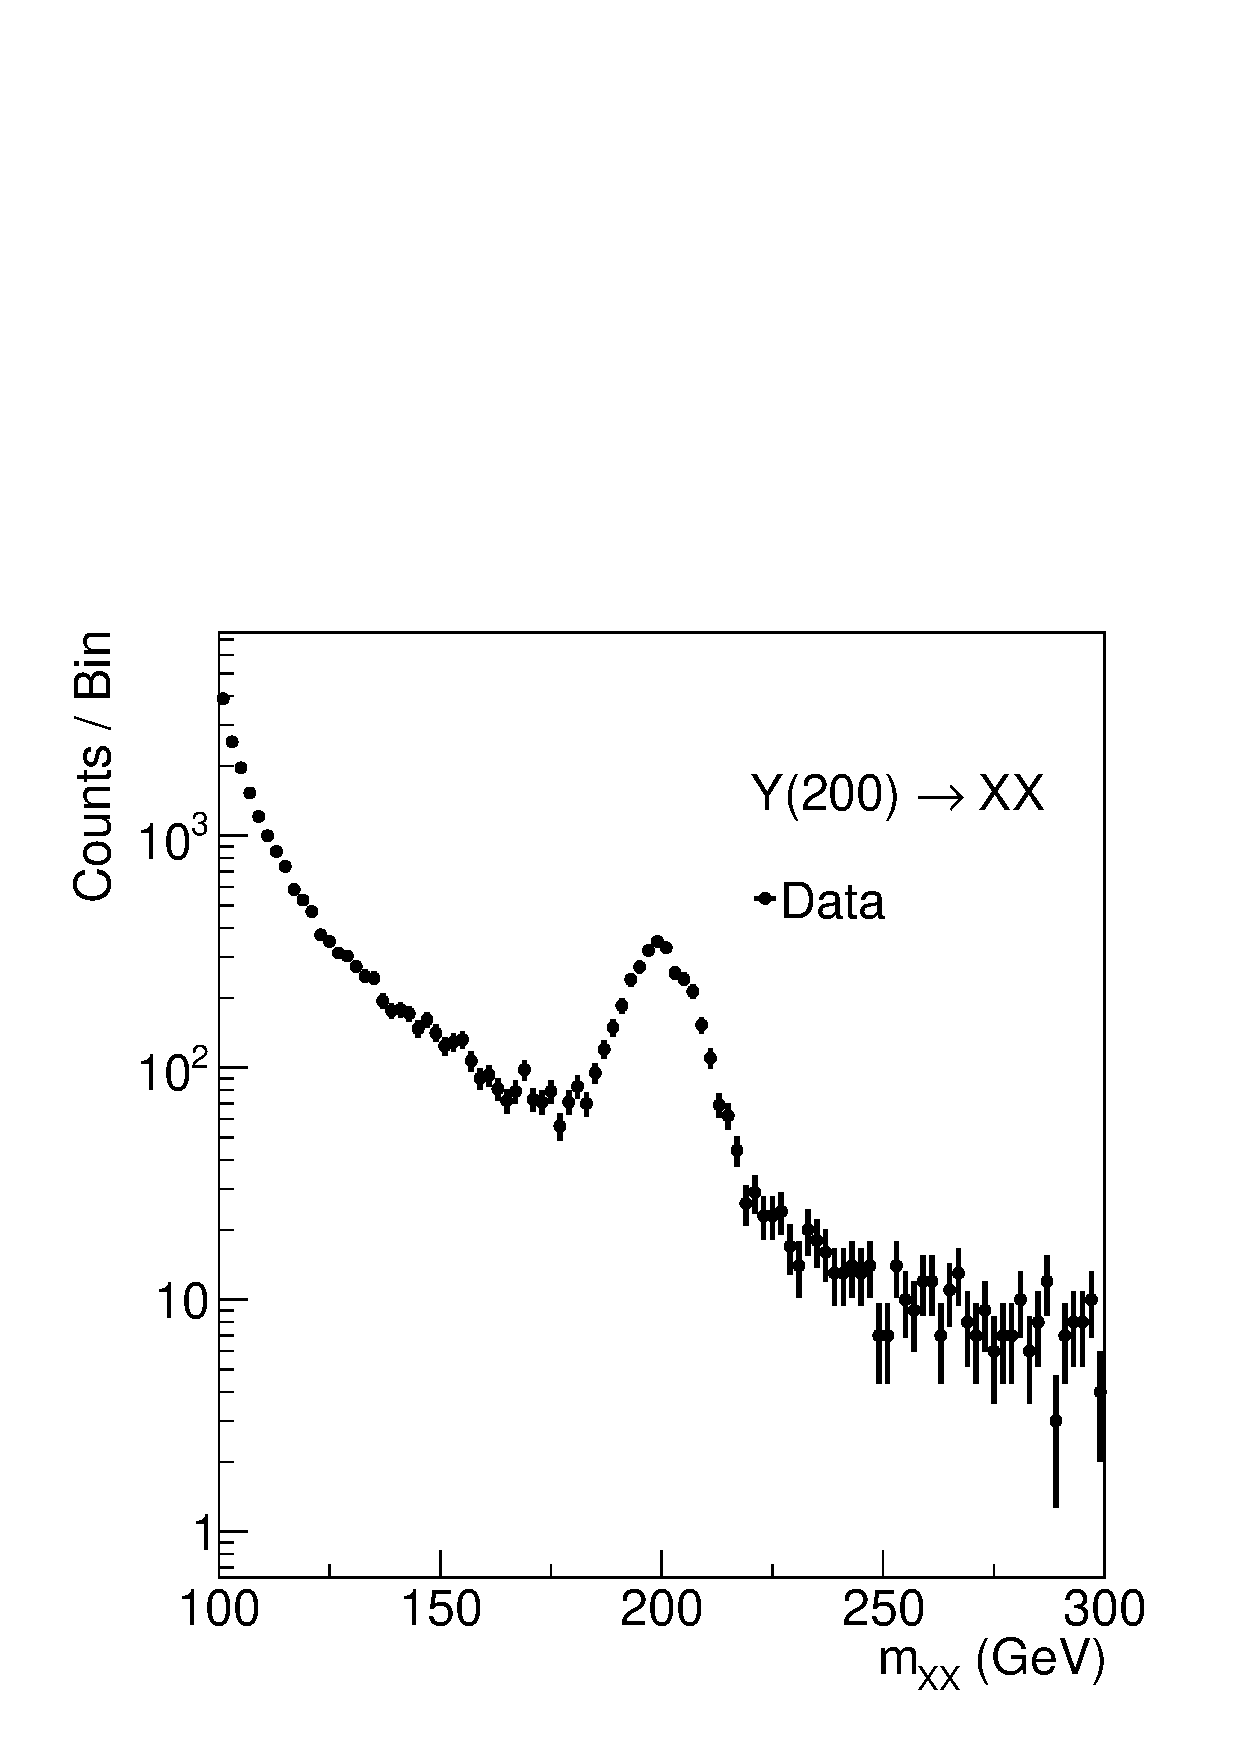
\includegraphics[page=1,width=\textwidth]{/home/kpapad/UG_thesis/Thesis/Analysis/out/Plots/WPhiJets_M200M100300_Application_MassSpectrum.pdf}
\end{figure}
\end{column}
\end{columns}
\end{frame}

\begin{frame}[label={sec:org0c06964}]{Fit based approach: Signal Fitting}
There is no point in trying to fit the really extreme smearing cases
\begin{columns}
\begin{column}{0.5\columnwidth}
\begin{figure}[h]
\centering
\includegraphics[page=6,width=\linewidth]{/home/kpapad/UG_thesis/Thesis/Analysis/src/WPhiJets_M200M100300_FitALL.pdf}
\end{figure}
\end{column}

\begin{column}{0.5\columnwidth}
\begin{figure}[h]
\centering
\includegraphics[page=7,width=\linewidth]{/home/kpapad/UG_thesis/Thesis/Analysis/src/WPhiJets_M200M100300_FitALL.pdf}
\end{figure}
\end{column}
\end{columns}
\end{frame}

\begin{frame}[label={sec:orgd671782}]{Fit based approach: Signal Fitting}
\begin{figure}[h]
\centering
\includegraphics[page=8,width=0.55\textwidth]{/home/kpapad/UG_thesis/Thesis/Analysis/src/WPhiJets_M200M100300_FitALL.pdf}
\end{figure}
\end{frame}

\begin{frame}[label={sec:org76caa09}]{Fit based approach: Signal from background separation}
Working in the nominal case, we scan the ranges \(m=\pm \frac{n}{2}\sigma\text{, }n=1, 2, 3, 4, 5, 6\) 
\begin{figure}[h]
\centering
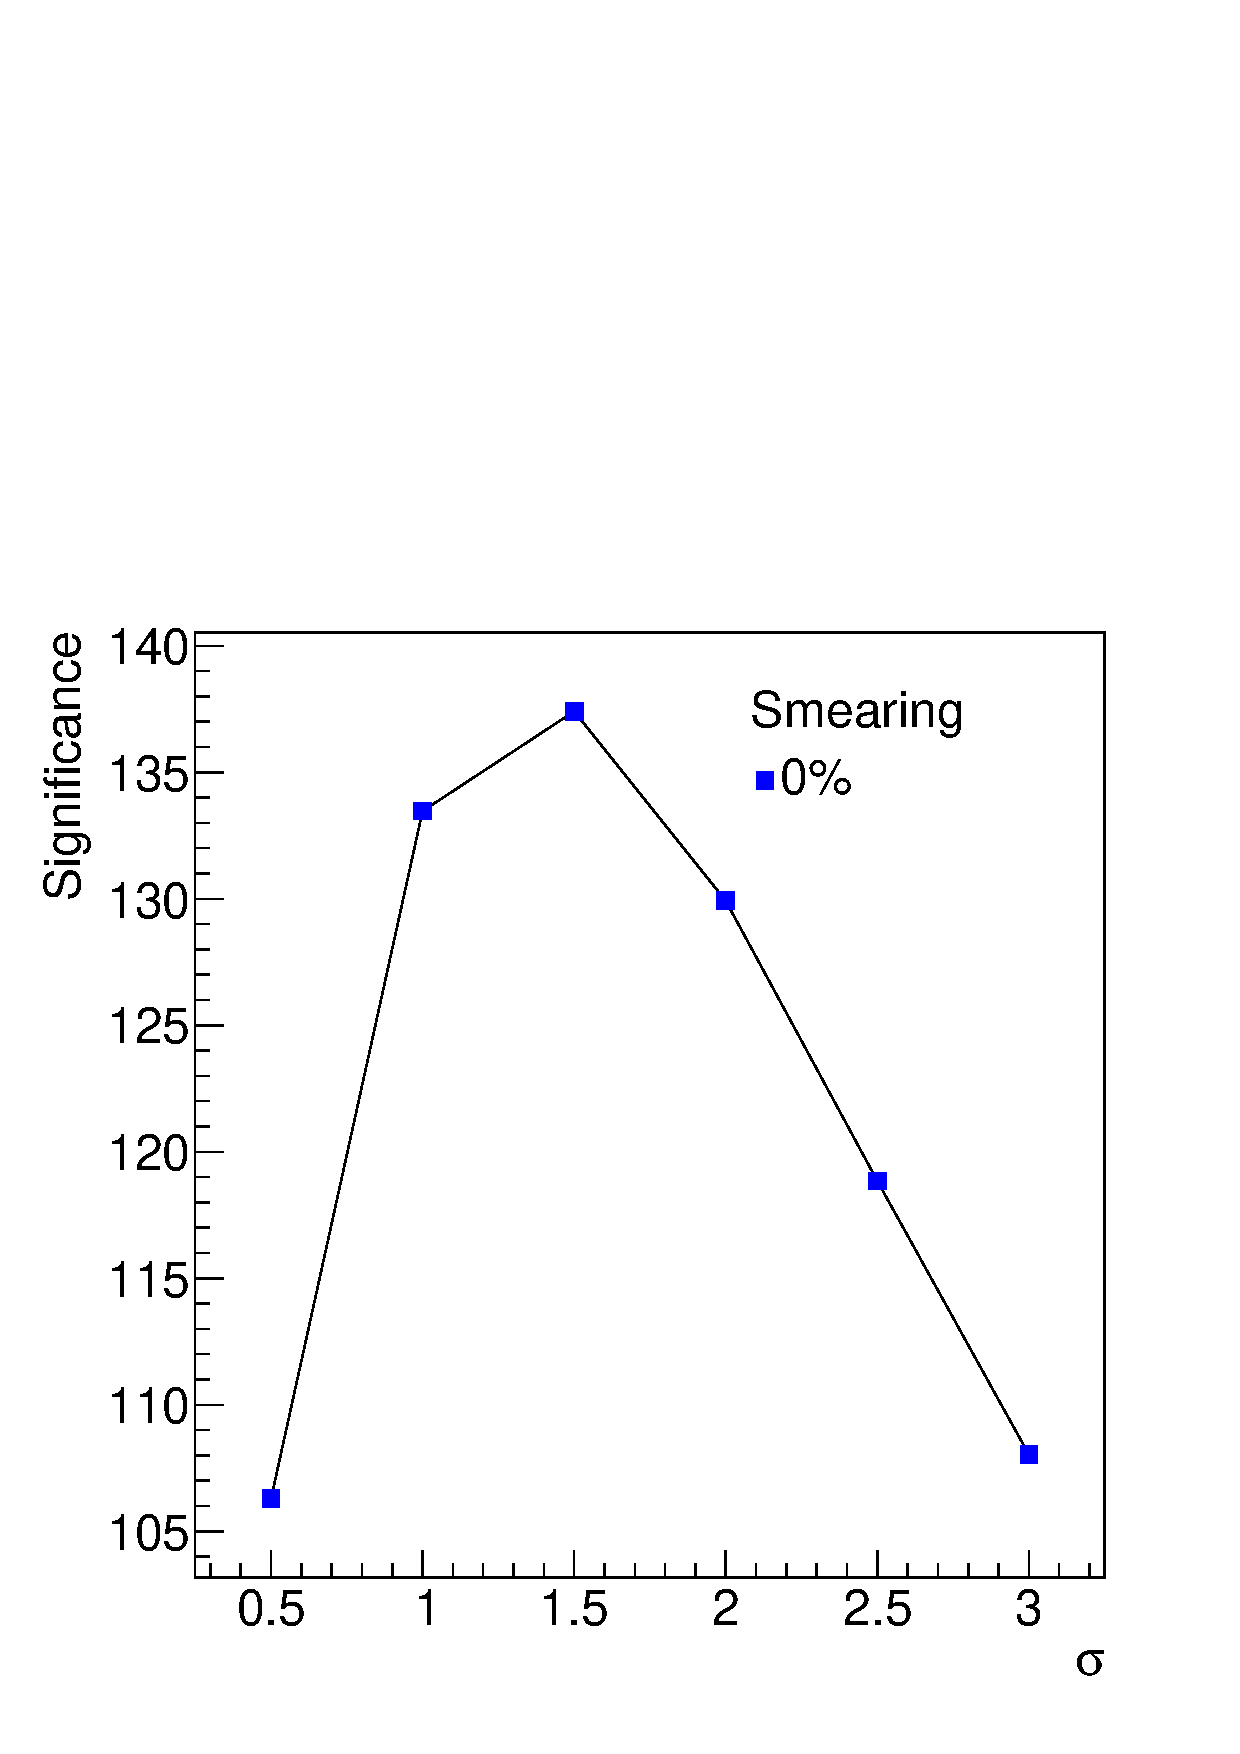
\includegraphics[page=1,width=0.45\textwidth]{/home/kpapad/UG_thesis/Thesis/Analysis/src/WPhiJets_M200M100300_Significance0.pdf}
\end{figure}
\end{frame}
\begin{frame}[label={sec:org137f31e}]{Fit based approach: Signal from background separation}
The best significance is in the \(\pm 1.5\sigma\) range. 
\begin{columns}
\begin{column}{0.5\columnwidth}
\begin{itemize}
\item fixed window
\item adaptive window
\end{itemize}
\end{column}
\begin{column}{0.5\columnwidth}
\begin{figure}[h]
\centering
\includegraphics[page=3,width=0.9\textwidth]{/home/kpapad/UG_thesis/Thesis/Bdt/src/WPhiJets_M200M100300_Significance.pdf}
\end{figure}
\end{column}
\end{columns}
\end{frame}
\begin{frame}[label={sec:orgbdb67f3}]{BDT approach: Feature space}
We use the same feature space as with the light mass search
\begin{figure}[h!]
\centering
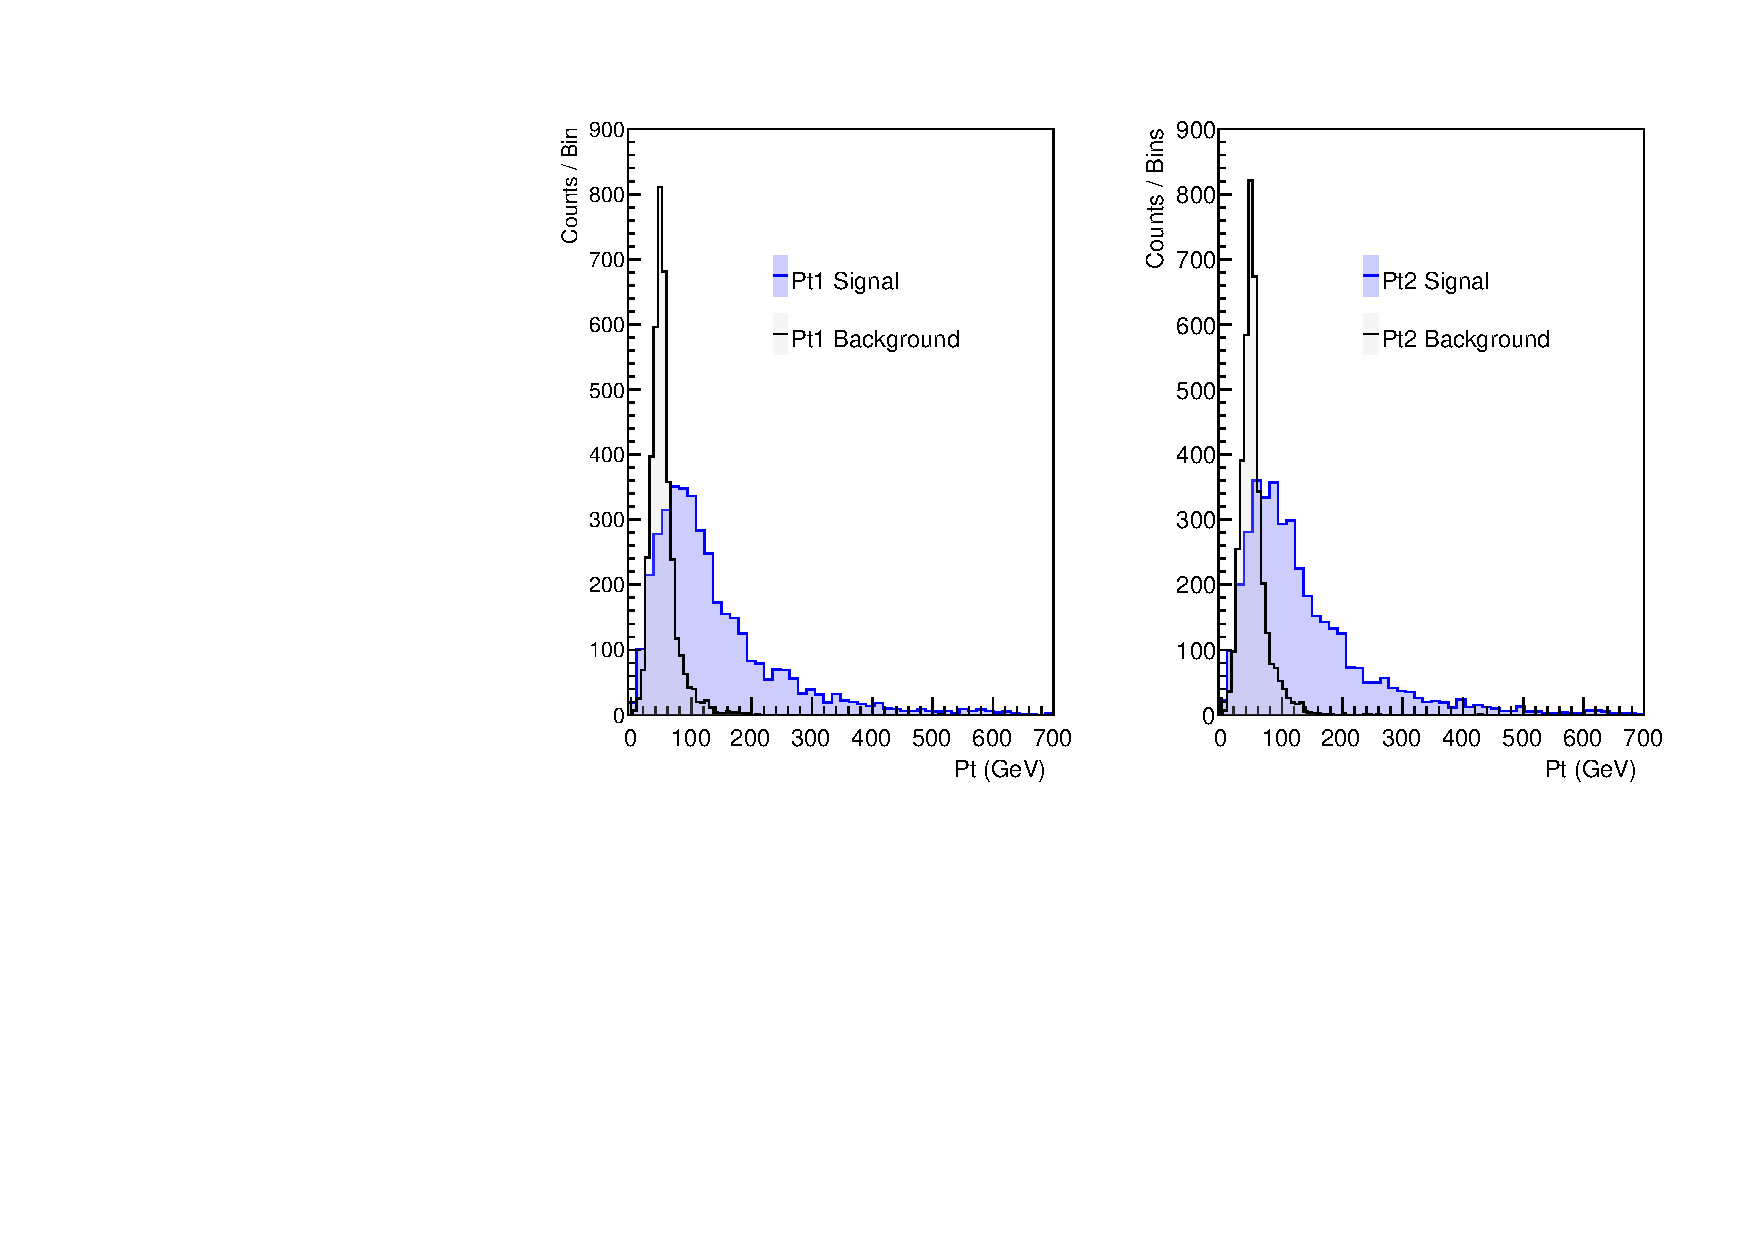
\includegraphics[page=1,width=0.9\textwidth]{/home/kpapad/UG_thesis/Thesis/Analysis/out/Plots/WPhiJets_M200M100300Deltas_varsplot.pdf}
\end{figure}
\end{frame}
\begin{frame}[label={sec:org0069914}]{BDT approach: Feature space}
\begin{figure}[h!]
\centering
\includegraphics[page=2,width=0.9\textwidth]{/home/kpapad/UG_thesis/Thesis/Analysis/out/Plots/WPhiJets_M200M100300Deltas_varsplot.pdf}
\end{figure}
\end{frame}

\begin{frame}[label={sec:orgfe04a91}]{BDT approach: The model}
\begin{columns}
\begin{column}{0.5\columnwidth}
\begin{itemize}
\item Trained with approximately 3K events
\item To examine overfitting we compare the ratio of training events to testing for each BDT score
\end{itemize}
\end{column}
\begin{column}{0.5\columnwidth}
  \begin{figure}[h!]
\centering
\includegraphics[page=5, width=\linewidth]{/home/kpapad/UG_thesis/Thesis/Bdt/out/Plots/WPhiJets_M200M100300DeltasPConf12BDTplot.pdf}
\end{figure}
\end{column}
\end{columns}
\end{frame}

\begin{frame}[label={sec:org86e3948}]{BDT approach: Signal from background separation}
\alert{Where should we place the cut?}
\begin{columns}
\begin{column}{0.5\columnwidth}
\begin{itemize}
\item We scan the whole BDT range to find the best region of interest
\item Best cut --> BDT score = 0.98.
\item This is rather tight, let's see what happens if we place a more relaxed cut at 0.86
\end{itemize}
\end{column}
\begin{column}{0.5\columnwidth}
\begin{figure}
\centering
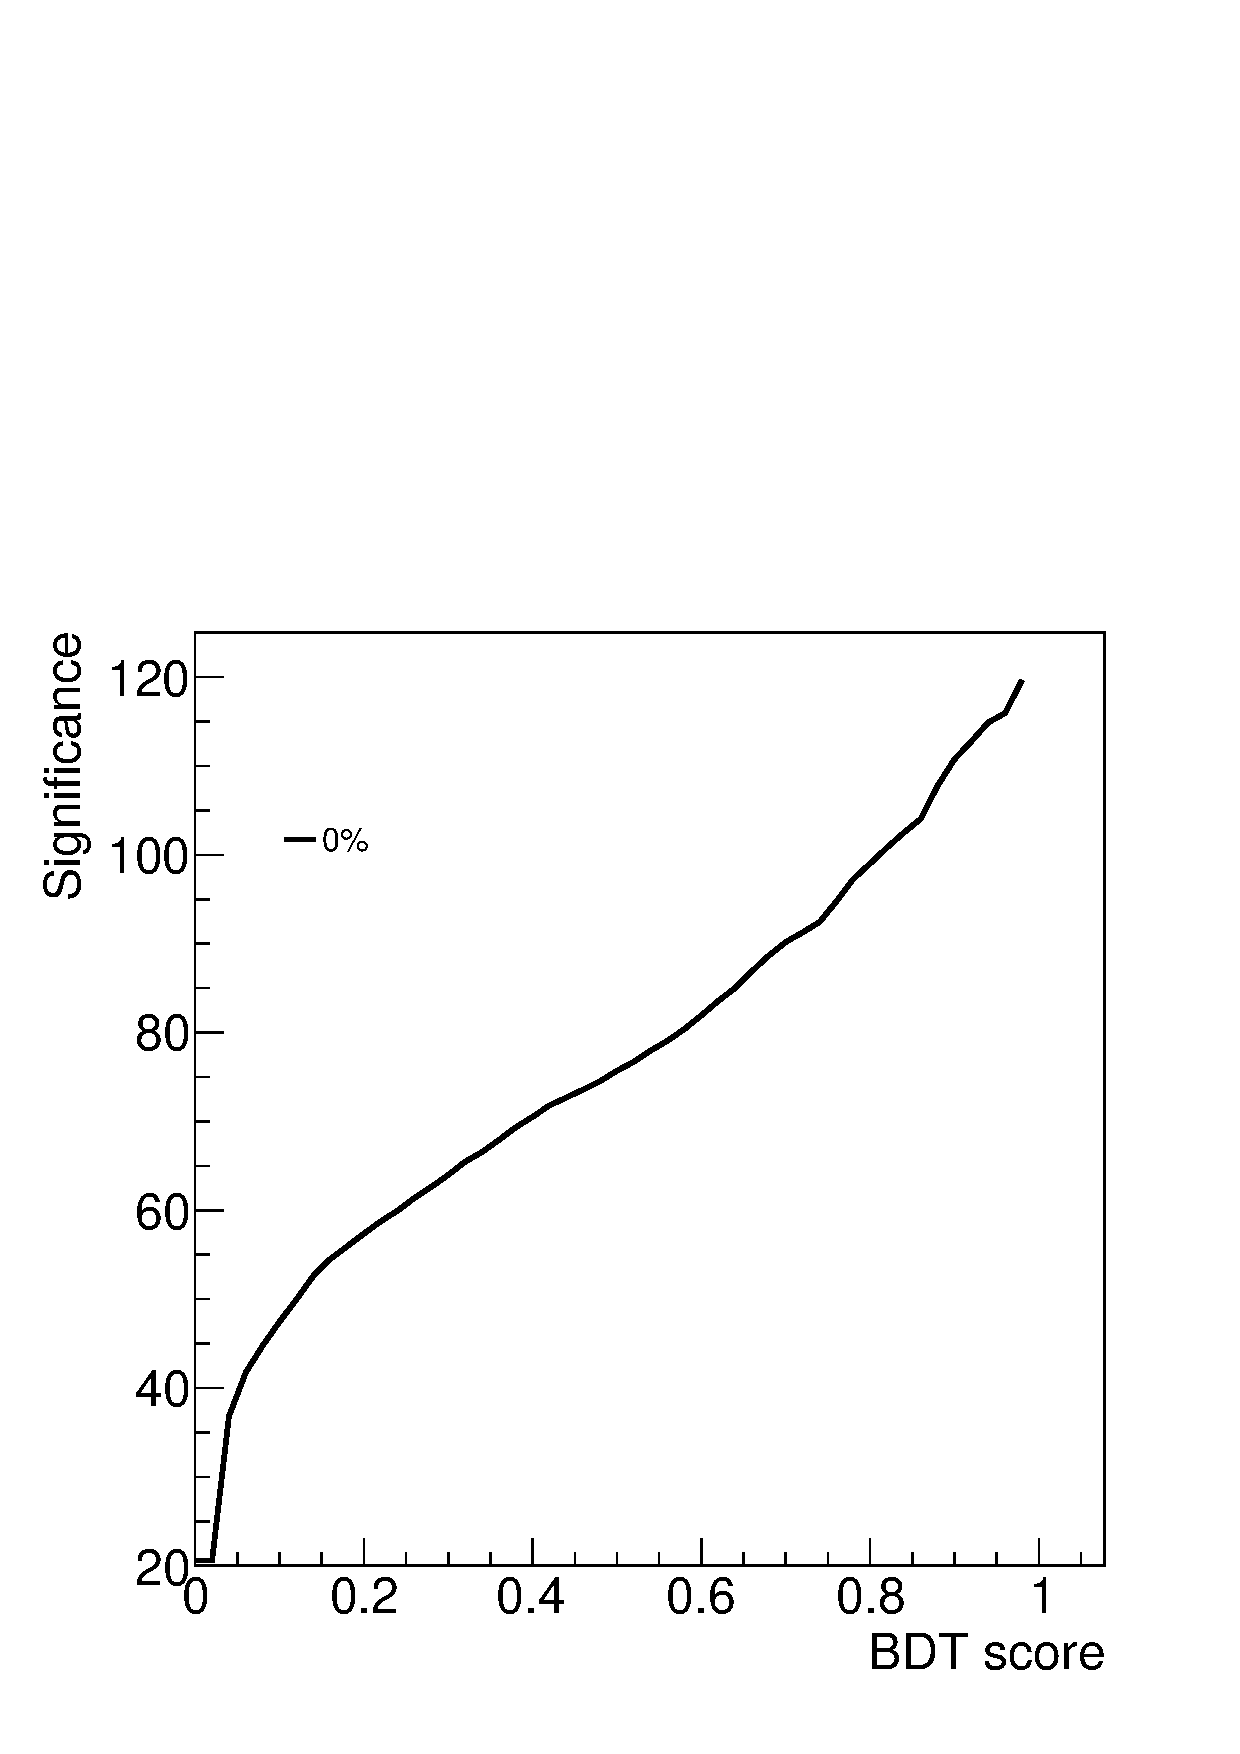
\includegraphics[page=1,width=\linewidth]{/home/kpapad/UG_thesis/Thesis/Bdt/src/WPhiJets_M200M100300_Significance0bdt.pdf}
\end{figure}
\end{column}
\end{columns}
\end{frame}
\begin{frame}[label={sec:org6e47759}]{BDT approach: Signal from background separation}
\begin{columns}
\begin{column}{0.5\columnwidth}
\begin{itemize}
\item The performance of the more relaxed cut is not as good as the best cut
\item The BDT model is rather robust
\end{itemize}
\end{column}
\begin{column}{0.5\columnwidth}
\begin{figure}
\centering
\includegraphics[page=2,width=\textwidth]{/home/kpapad/UG_thesis/Thesis/Bdt/src/WPhiJets_M200M100300_Significance.pdf}
\end{figure}
\end{column}
\end{columns}
\end{frame}
\begin{frame}[label={sec:org4d43ecc}]{Synopsis}
\begin{columns}
\begin{column}{0.5\columnwidth}
\begin{itemize}
\item The performance of the BDT and Fit are comparable when smeaing is mild
\item Fit performance drops dramatically
\item BDT is more robust
\end{itemize}
\end{column}

\begin{column}{0.5\columnwidth}
\begin{figure}
\centering
\includegraphics[page=4,width=\textwidth]{/home/kpapad/UG_thesis/Thesis/Bdt/src/WPhiJets_M200M100300_Significance.pdf}
\end{figure}
\end{column}
\end{columns}
\end{frame}

\section{Results}
\label{sec:orgca35bba}
\begin{frame}[label={sec:orgca98d5c}]{Results}
\begin{columns}
\begin{column}{0.5\columnwidth}
\begin{itemize}
\item Light \(Y \rightarrow XX\)
\end{itemize}
\begin{figure}
\centering
\includegraphics[page=4,width=\textwidth]{/home/kpapad/UG_thesis/Thesis/Bdt/src/WPhiJets_M60M5080_Significance.pdf}
\end{figure}
\end{column}

\begin{column}{0.5\columnwidth}
\begin{itemize}
\item Heavy \(Y \rightarrow XX\)
\end{itemize}
\begin{figure}
\centering
\includegraphics[page=4,width=\textwidth]{/home/kpapad/UG_thesis/Thesis/Bdt/src/WPhiJets_M200M100300_Significance.pdf}
\end{figure}
\end{column}
\end{columns}
\end{frame}

\begin{frame}[label={sec:org7fbeae6}]{Results}
Overall, the BDT is more robust as it learns features that do not get affected by energy scale uncertainties\newline

\alert{So is the BDT better?}
\begin{itemize}
\item No: A more careful event selection can improve the performance of the fit based analysis
\item yes: In the presence of energy scale uncertainties, the fit based analysis reaches a "breaking point"
\end{itemize}
\end{frame}

\section{Unused stuff}
\label{sec:orge0d2938}
\begin{frame}[label={sec:org1222400}]{Backup}
\alert{Welcome to the backup slides!}
\end{frame}


\begin{frame}[label={sec:orgc157cde}]{Supervised Learning}
\begin{itemize}
\item The model is trained using training data
\item The trained model is tested using testing data
\item If we like the resulting model, we apply it!\linebreak
\end{itemize}

\alert{\ldots{}but what is this model?}
\begin{itemize}
\item A function that given the input feautres x, it returns the probability x being class A
\item The goal of the training is to minimize the difference between the predicted output \(y_{i} \in [0, 1]\) and the real output \(\hat{y_{i}} = 0\text{ class B, or }\hat{y_{i}} = 1\text{ class A}\)
\end{itemize}
\end{frame}
\begin{frame}[label={sec:org72f55b7}]{BDT 1a: Boosted decision trees}
In this study the model of choice is Boosted Decision Trees(BDT).
\begin{itemize}
\item It classifies data using decision tree models
\end{itemize}
\begin{figure}[h]
\centering
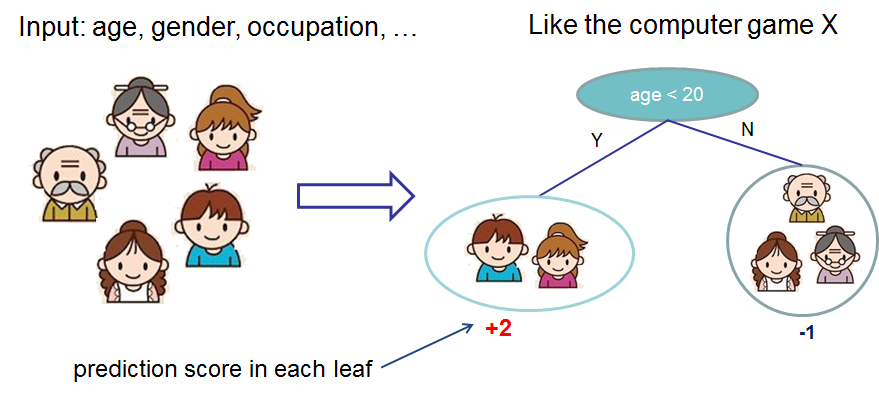
\includegraphics[width=0.85 \textwidth, ext=.png type=png]{/home/kpapad/UG_thesis/Thesis/Dissertation/Presentation/figures/cart.png}
\end{figure}
\end{frame}
\begin{frame}[label={sec:orge22b3dd}]{BDT 2b: Boosted Decision Trees}
Usually only one tree is not powerful enough --> Use  more trees in additive manner(Boosting)
\begin{figure}[h]
\centering
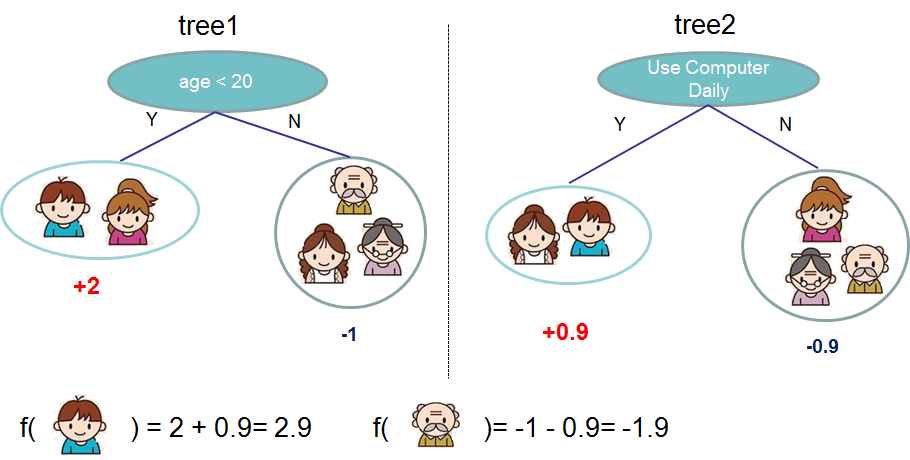
\includegraphics[width=0.85 \textwidth, ext=.png type=png]{/home/kpapad/UG_thesis/Thesis/Dissertation/Presentation/figures/twocart.png}
\end{figure}
\end{frame}
\begin{frame}[label={sec:orga03c000}]{BDT 3: Signal from background separation}
Where should we place the cut in order to accpet most most of the  signal while rejecting most of background?
\begin{figure}[hb]
\centering
\includegraphics[page=2, width=0.85 \textwidth, ext=.png type=jpg]{/home/kpapad/UG_thesis/Thesis/Bdt/out/Plots/WPhiJets_M60M5080DeltasPConf12BDTplot.pdf}
\end{figure}
\end{frame}

\begin{frame}[label={sec:org335f636}]{Fit based signal from background separation}
We can count the signal and background events, in a region of interest \(I\):
\begin{align}
O &= \int_{I} observation(x) dx \\
B &= \int_{I} bkg(x) dx\\
S &= O - B
\end{align}
\end{frame}
\begin{frame}[label={sec:org963ef61}]{Fit based approach: Background Fitting light}
\begin{columns}
\begin{column}{0.5\columnwidth}
\begin{itemize}
\item To simplify things a bit, we fit the background sepratelly
\item The background shape is kept constant throughout the fits
\item Shape: \(\alpha + \beta x + \gamma x^2 + \delta x^3\)
\end{itemize}
\end{column}
\begin{column}{0.5\columnwidth}
\begin{figure}[h]
\centering
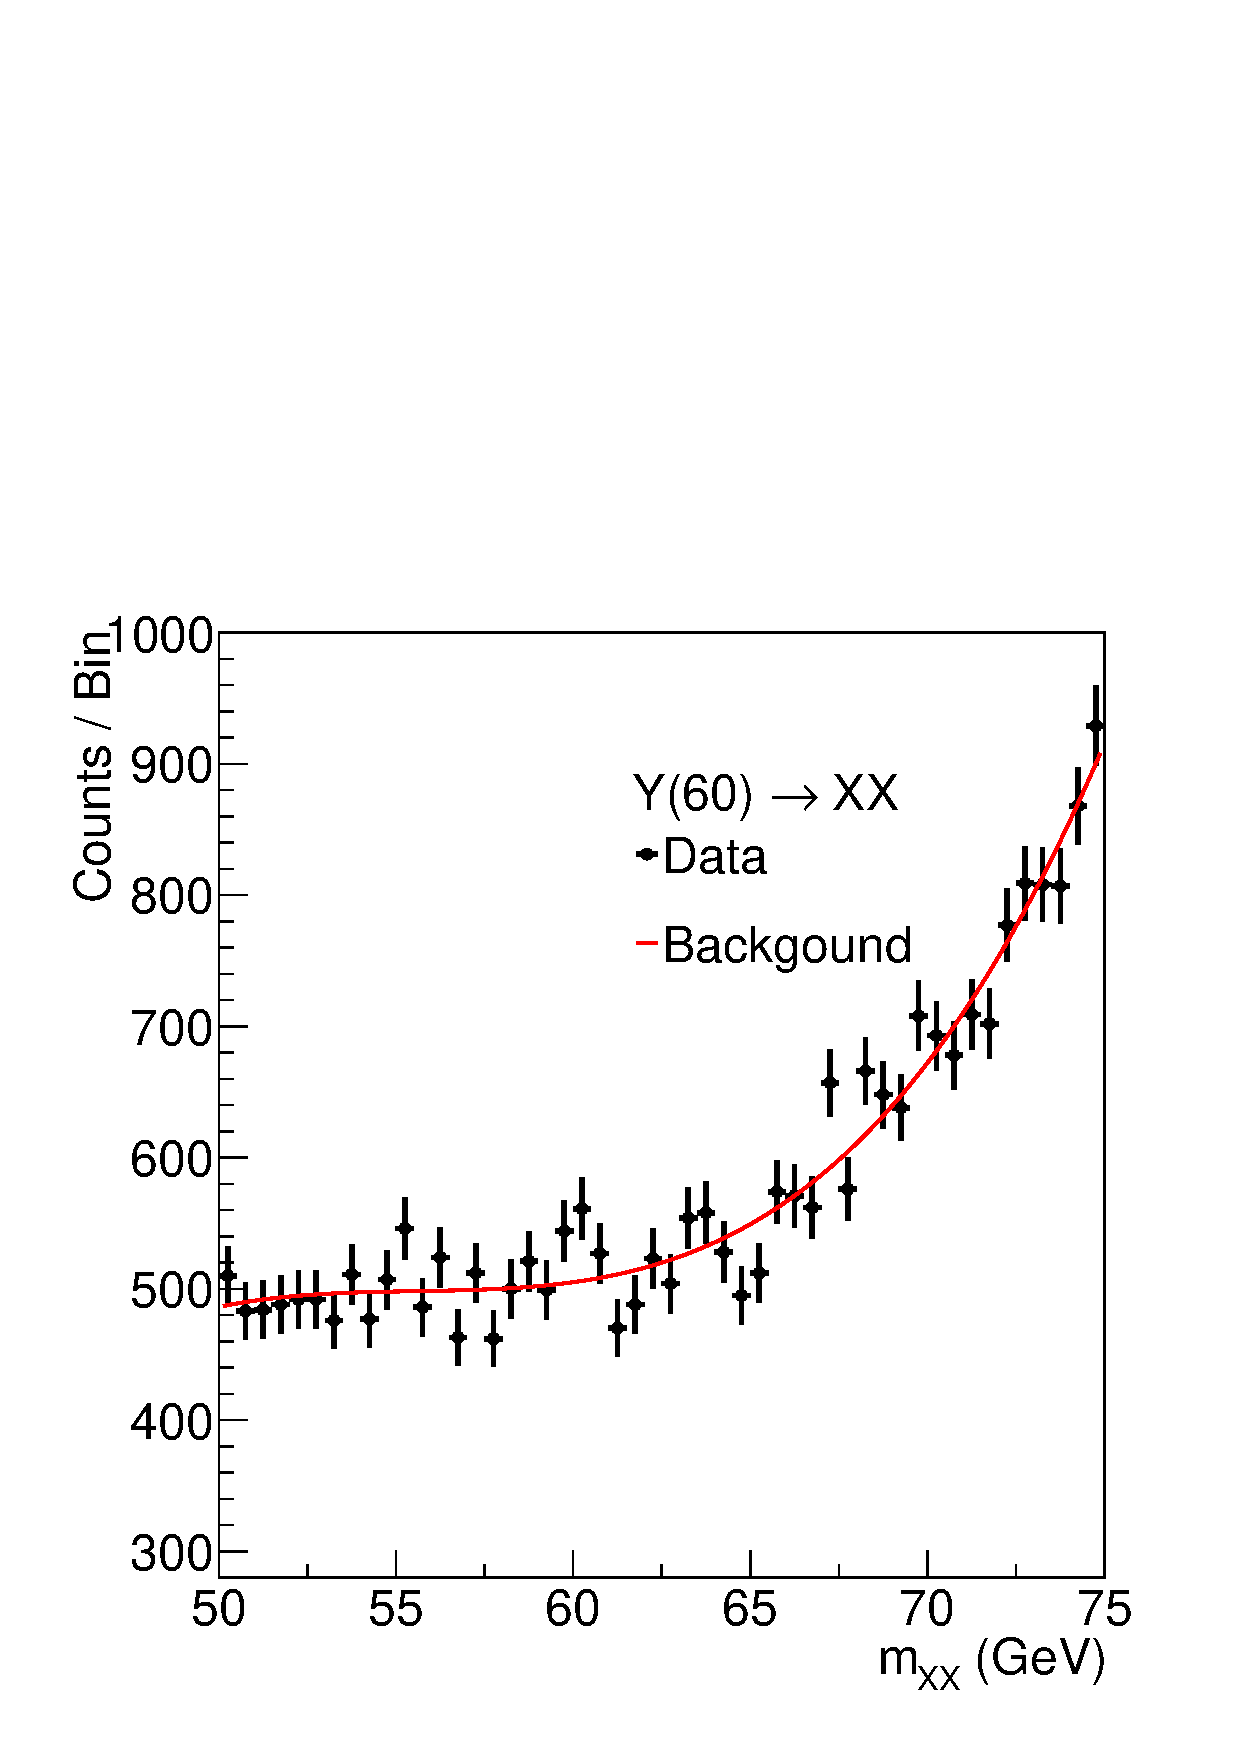
\includegraphics[page=1,width=\textwidth]{/home/kpapad/UG_thesis/Thesis/Analysis/out/Plots/WPhiJets_M60M5080_Application_bkgonly_Fit.pdf}
\end{figure}
\end{column}
\end{columns}
\end{frame}

\begin{frame}[label={sec:org20be653}]{Fit based approach: Background Fitting}
\begin{columns}
\begin{column}{0.5\columnwidth}
\begin{itemize}
\item The background shape is kept constant
\item Shape: \(\alpha + \beta x^{-1/2} + \gamma x^{-1} + \delta x^{3/2}\)
\end{itemize}
\end{column}
\begin{column}{0.5\columnwidth}
\begin{figure}[h]
\centering
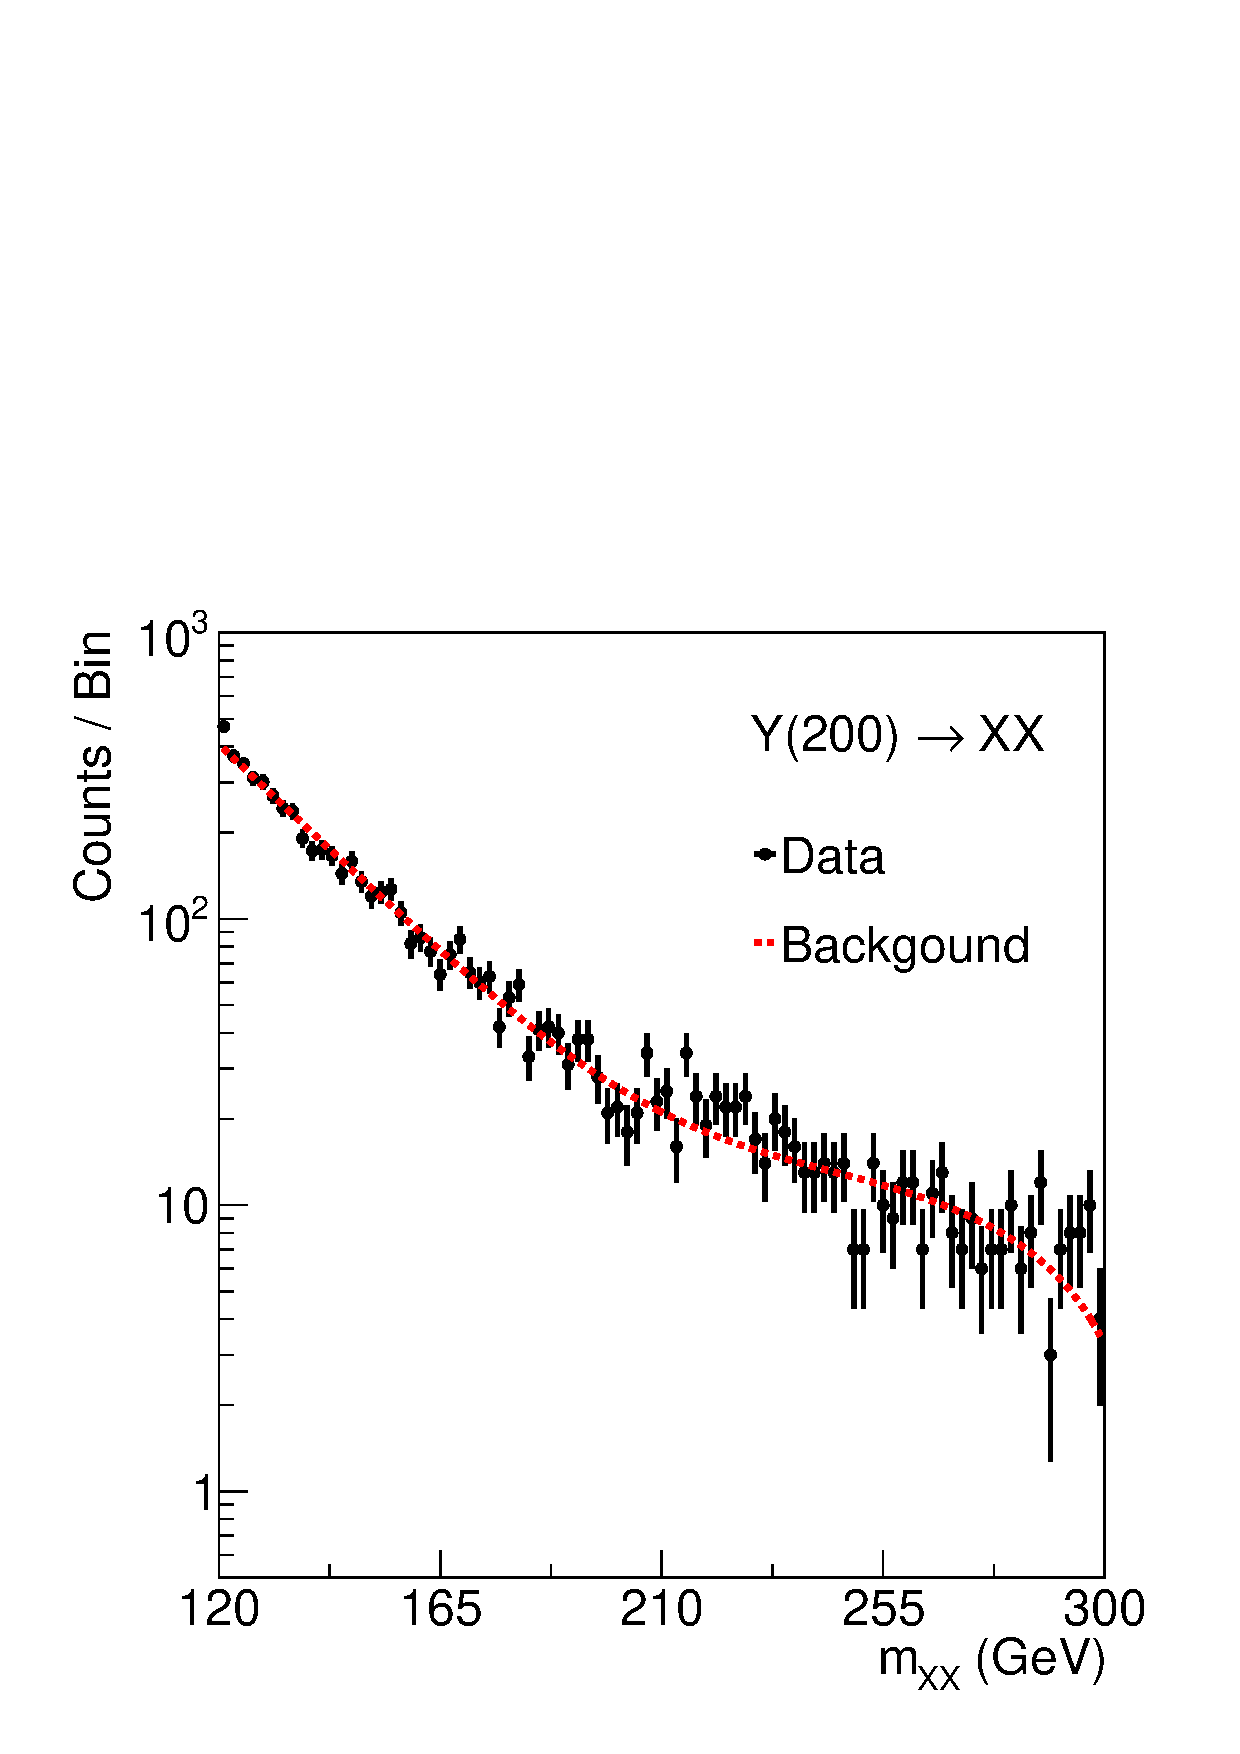
\includegraphics[page=1,width=\textwidth]{/home/kpapad/UG_thesis/Thesis/Analysis/out/Plots/WPhiJets_M200M100300_Application_bkgFit.pdf}
\end{figure}
\end{column}
\end{columns}
\end{frame}


\begin{frame}[label={sec:org00a8127}]{Fit based approach: Signal Fitting}
Then we proceed and fit the signal
\begin{columns}
\begin{column}{0.5\columnwidth}
\begin{figure}[h]
\centering
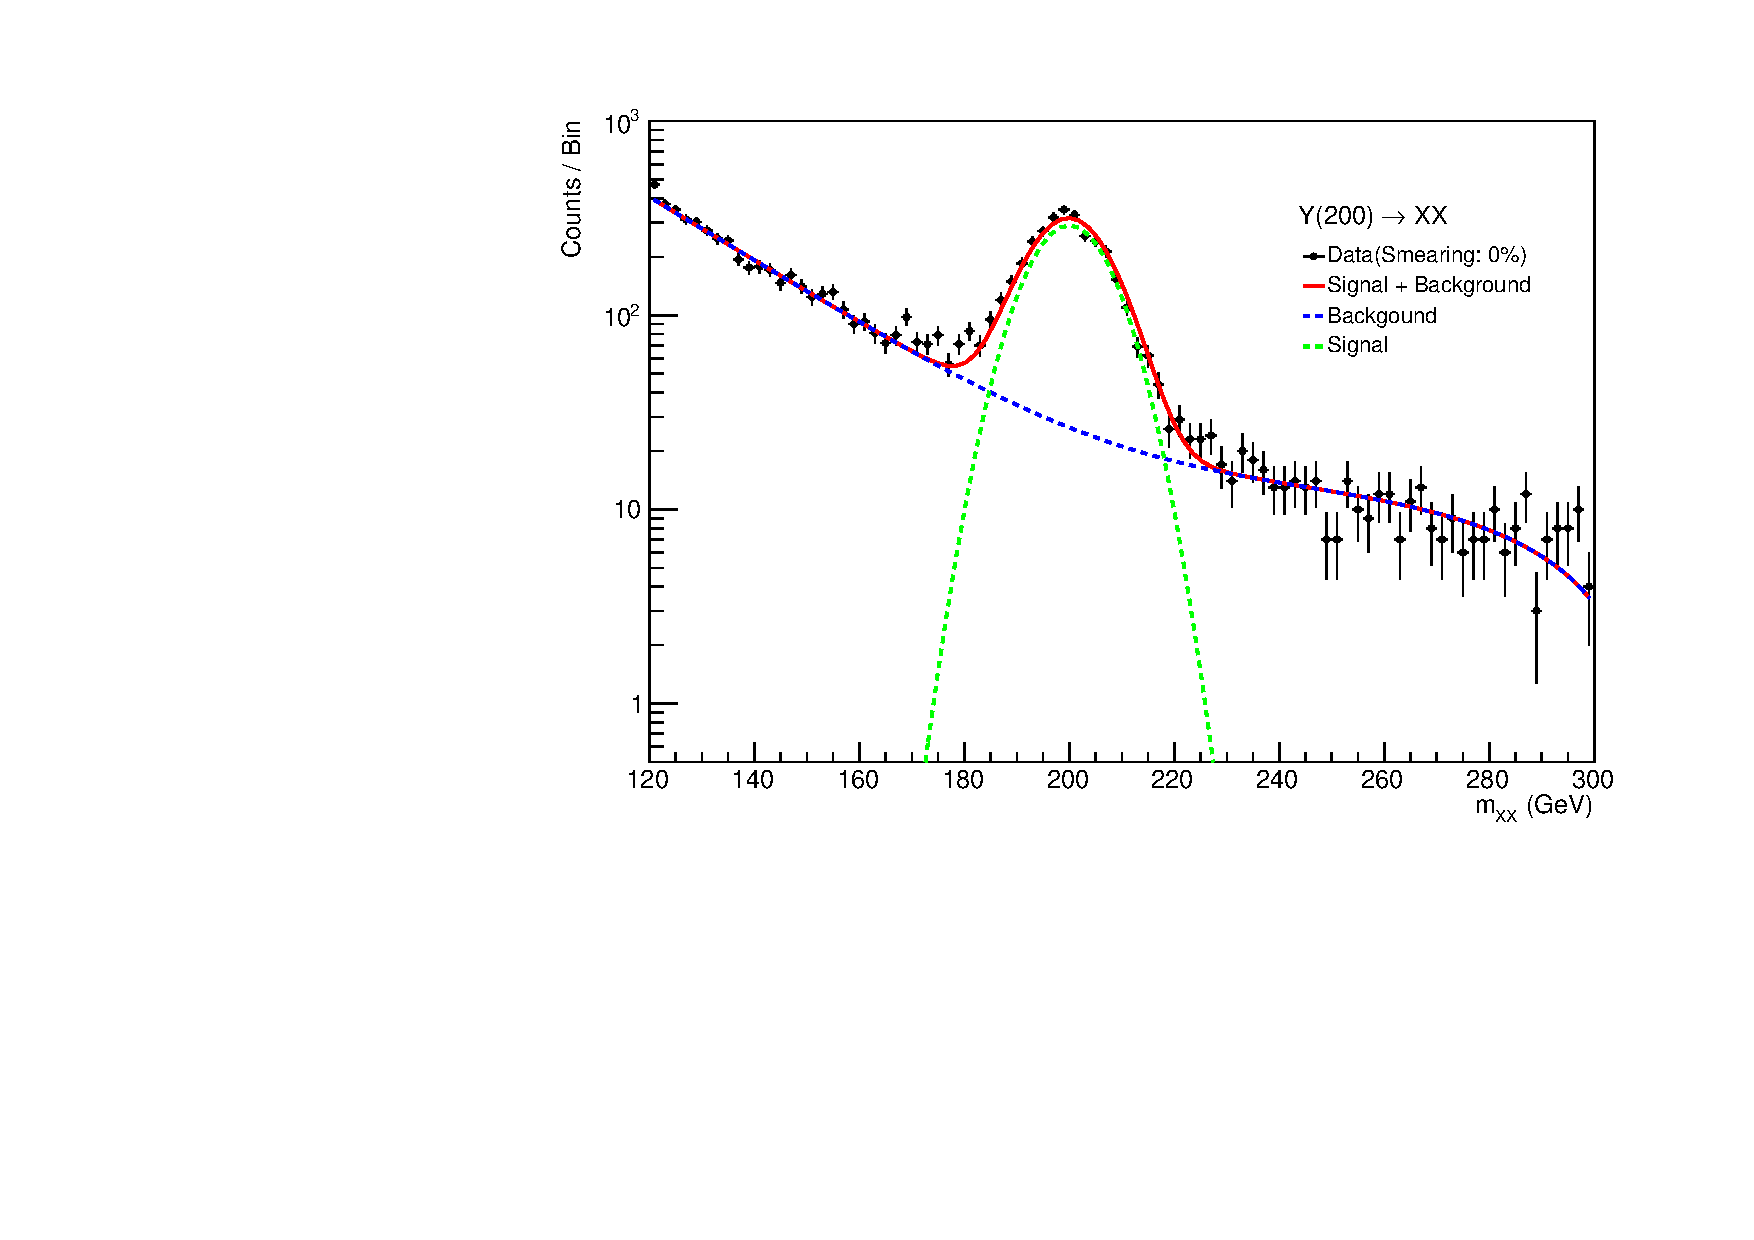
\includegraphics[page=1,width=\linewidth]{/home/kpapad/UG_thesis/Thesis/Analysis/src/WPhiJets_M200M100300_FitALL.pdf}
\end{figure}
\end{column}

\begin{column}{0.5\columnwidth}
\begin{figure}[h]
\centering
\includegraphics[page=2,width=\linewidth]{/home/kpapad/UG_thesis/Thesis/Analysis/src/WPhiJets_M200M100300_FitALL.pdf}
\end{figure}
\end{column}
\end{columns}
\end{frame}

\begin{frame}[label={sec:org262762f}]{Fit based approach: Signal Fitting}
\begin{columns}
\begin{column}{0.5\columnwidth}
\begin{figure}[h]
\centering
\includegraphics[page=3,width=\linewidth]{/home/kpapad/UG_thesis/Thesis/Analysis/src/WPhiJets_M200M100300_FitALL.pdf}
\end{figure}
\end{column}

\begin{column}{0.5\columnwidth}
\begin{figure}[h]
\centering
\includegraphics[page=4,width=\linewidth]{/home/kpapad/UG_thesis/Thesis/Analysis/src/WPhiJets_M200M100300_FitALL.pdf}
\end{figure}
\end{column}
\end{columns}
\end{frame}

\begin{frame}[label={sec:orgf22f234}]{Fit based approach: Signal Fitting}
\begin{figure}[h]
\centering
\includegraphics[page=5,width=0.55\textwidth]{/home/kpapad/UG_thesis/Thesis/Analysis/src/WPhiJets_M200M100300_FitALL.pdf}
\end{figure}
\end{frame}


\begin{frame}[label={sec:orgceeb587}]{BDT approach: Application}
Feed the application set to the BDT --> BDT plots
\begin{columns}
\begin{column}{0.5\columnwidth}
\begin{figure}[h]
\centering
\includegraphics[page=6,width=\linewidth]{/home/kpapad/UG_thesis/Thesis/Bdt/out/Plots/WPhiJets_M200M100300Deltas_Application12BDTplot.pdf}
\end{figure}
\end{column}
\begin{column}{0.5\columnwidth}
\begin{figure}[h]
\centering
\includegraphics[page=6,width=\linewidth]{/home/kpapad/UG_thesis/Thesis/Bdt/out/Plots/WPhiJets_M200M100300Deltas_Application_Smeared512BDTplot.pdf}
\end{figure}
\end{column}
\end{columns}
\end{frame}

\begin{frame}[label={sec:orgafbb629}]{BDT approach: Application}
\begin{columns}
\begin{column}{0.5\columnwidth}
\begin{figure}[h]
\centering
\includegraphics[page=6,width=\linewidth]{/home/kpapad/UG_thesis/Thesis/Bdt/out/Plots/WPhiJets_M200M100300Deltas_Application_Smeared1012BDTplot.pdf}
\end{figure}
\end{column}
\begin{column}{0.5\columnwidth}
\begin{figure}[h]
\centering
\includegraphics[page=6,width=\linewidth]{/home/kpapad/UG_thesis/Thesis/Bdt/out/Plots/WPhiJets_M200M100300Deltas_Application_Smeared1512BDTplot.pdf}
\end{figure}
\end{column}
\end{columns}
\end{frame}

\begin{frame}[label={sec:org5a25930}]{BDT approach: Application}
\begin{columns}
\begin{column}{0.5\columnwidth}
\begin{figure}[h]
\centering
\includegraphics[page=6,width=\linewidth]{/home/kpapad/UG_thesis/Thesis/Bdt/out/Plots/WPhiJets_M200M100300Deltas_Application_Smeared2012BDTplot.pdf}
\end{figure}
\end{column}
\begin{column}{0.5\columnwidth}
\begin{figure}[h]
\centering
\includegraphics[page=6,width=\linewidth]{/home/kpapad/UG_thesis/Thesis/Bdt/out/Plots/WPhiJets_M200M100300Deltas_Application_Smeared3012BDTplot.pdf}
\end{figure}
\end{column}
\end{columns}
\end{frame}

\begin{frame}[label={sec:org96ead05}]{BDT approach: Application}
\begin{columns}
\begin{column}{0.5\columnwidth}
\begin{figure}[h]
\centering
\includegraphics[page=6,width=\linewidth]{/home/kpapad/UG_thesis/Thesis/Bdt/out/Plots/WPhiJets_M200M100300Deltas_Application_Smeared4012BDTplot.pdf}
\end{figure}
\end{column}
\begin{column}{0.5\columnwidth}
\begin{figure}[h]
\centering
\includegraphics[page=6,width=\linewidth]{/home/kpapad/UG_thesis/Thesis/Bdt/out/Plots/WPhiJets_M200M100300Deltas_Application_Smeared5012BDTplot.pdf}
\end{figure}
\end{column}
\end{columns}
\end{frame}
\end{document}